\documentclass[11pt,a4paper]{article}
\usepackage[margin=25mm]{geometry}\usepackage{pdfpages,hyperref}
\pdfinclusioncopyfonts=1
\begin{document}
\begin{center}{\Large Higher-rank Suzuki geometries}\\[4mm]
{\large Complete source treatment and proofs for L110}\end{center}
This volume treats the fixed twenty-page higher-rank article. The opening
manuscript and claim ledger give the current disposition. Exact earlier
proofs retain their historical scope statements; the separate scalar
geometry supplement proves the stronger conclusion where indicated.
Two additional necessity papers repair the conditional-extension gap
identified in the retained review of the first assembly.
The final papers are reused common theory, with classical premises
explicitly attributed. No new original, principal-refutation count,
Lean formalization or compression measurement is claimed.\par\medskip
\small\begin{tabular}{rl}
2 & Source treatment and corrections\\
7 & The omitted pure-subfield boundary\\
10 & Prime-subfield residues do not extend\\
14 & Obstructions to five prescribed constructions\\
17 & Scalar fields and split families\\
20 & Necessity for split extensions\\
24 & Necessity for torus and pure-subfield extensions\\
29 & Field descent and compatible tori\\
36 & All prescribed torus parameters\\
40 & Pure subfields and the mixed scalar obstruction\\
45 & Diagrams of the surviving families\\
47 & Scalar subspaces give actual geometries\\
49 & Preliminary source statements\\
52 & The prime-degree obstruction\\
55 & Normalizer restrictions and embedded uniqueness\\
60 & Necessary prime-degree patterns\\
66 & Realizations of the rank-three patterns\\
71 & The omitted rank-three torus family\\
75 & The nonthin geometry over eight elements\\
78 & The nonthin geometry over thirty-two elements\\
80 & The earlier algebraic scalar family\\
83 & Scalar subspaces and central covers\\
87 & Common elementary Suzuki reductions\\
92 & The normalizer families\\
100 & Corrected subfield families\\
\end{tabular}\newpage
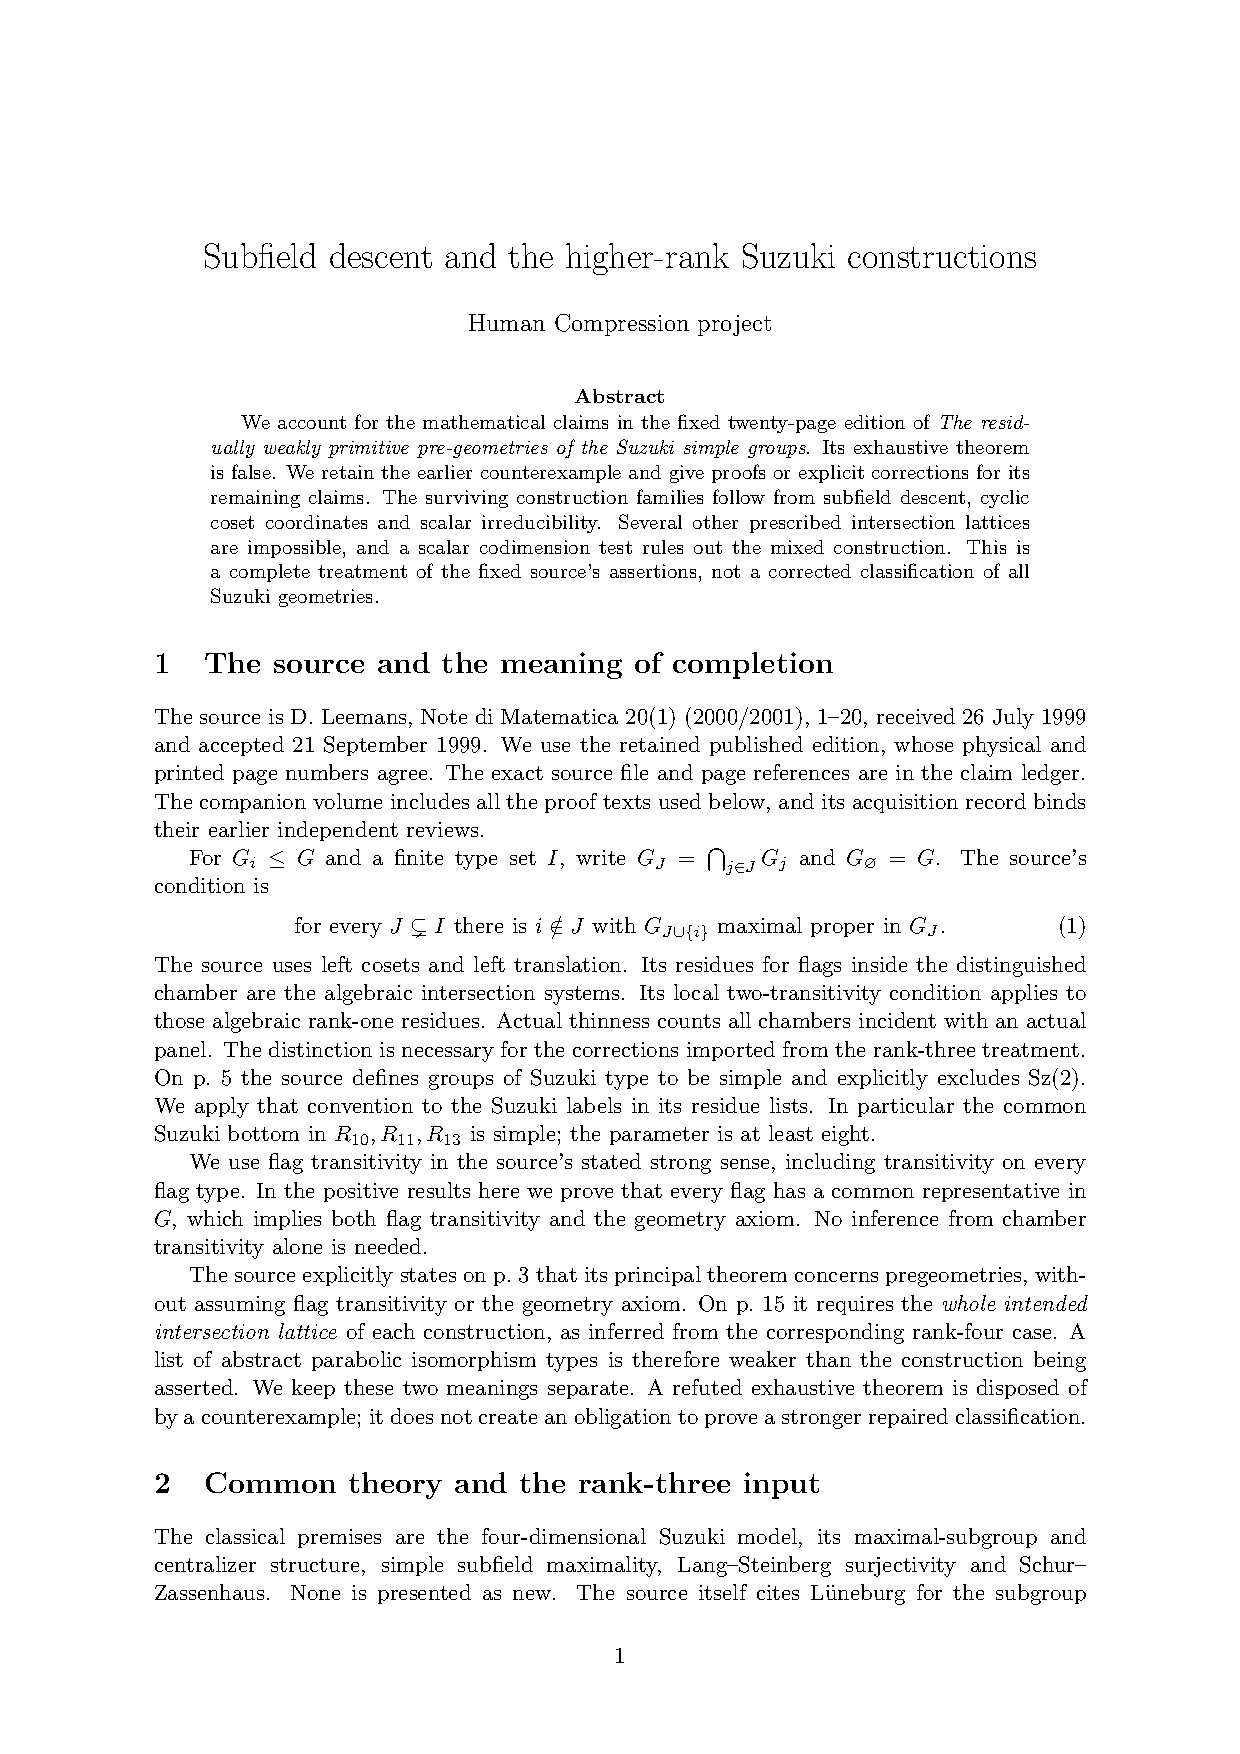
\includepdf[pages=-]{completion.pdf}
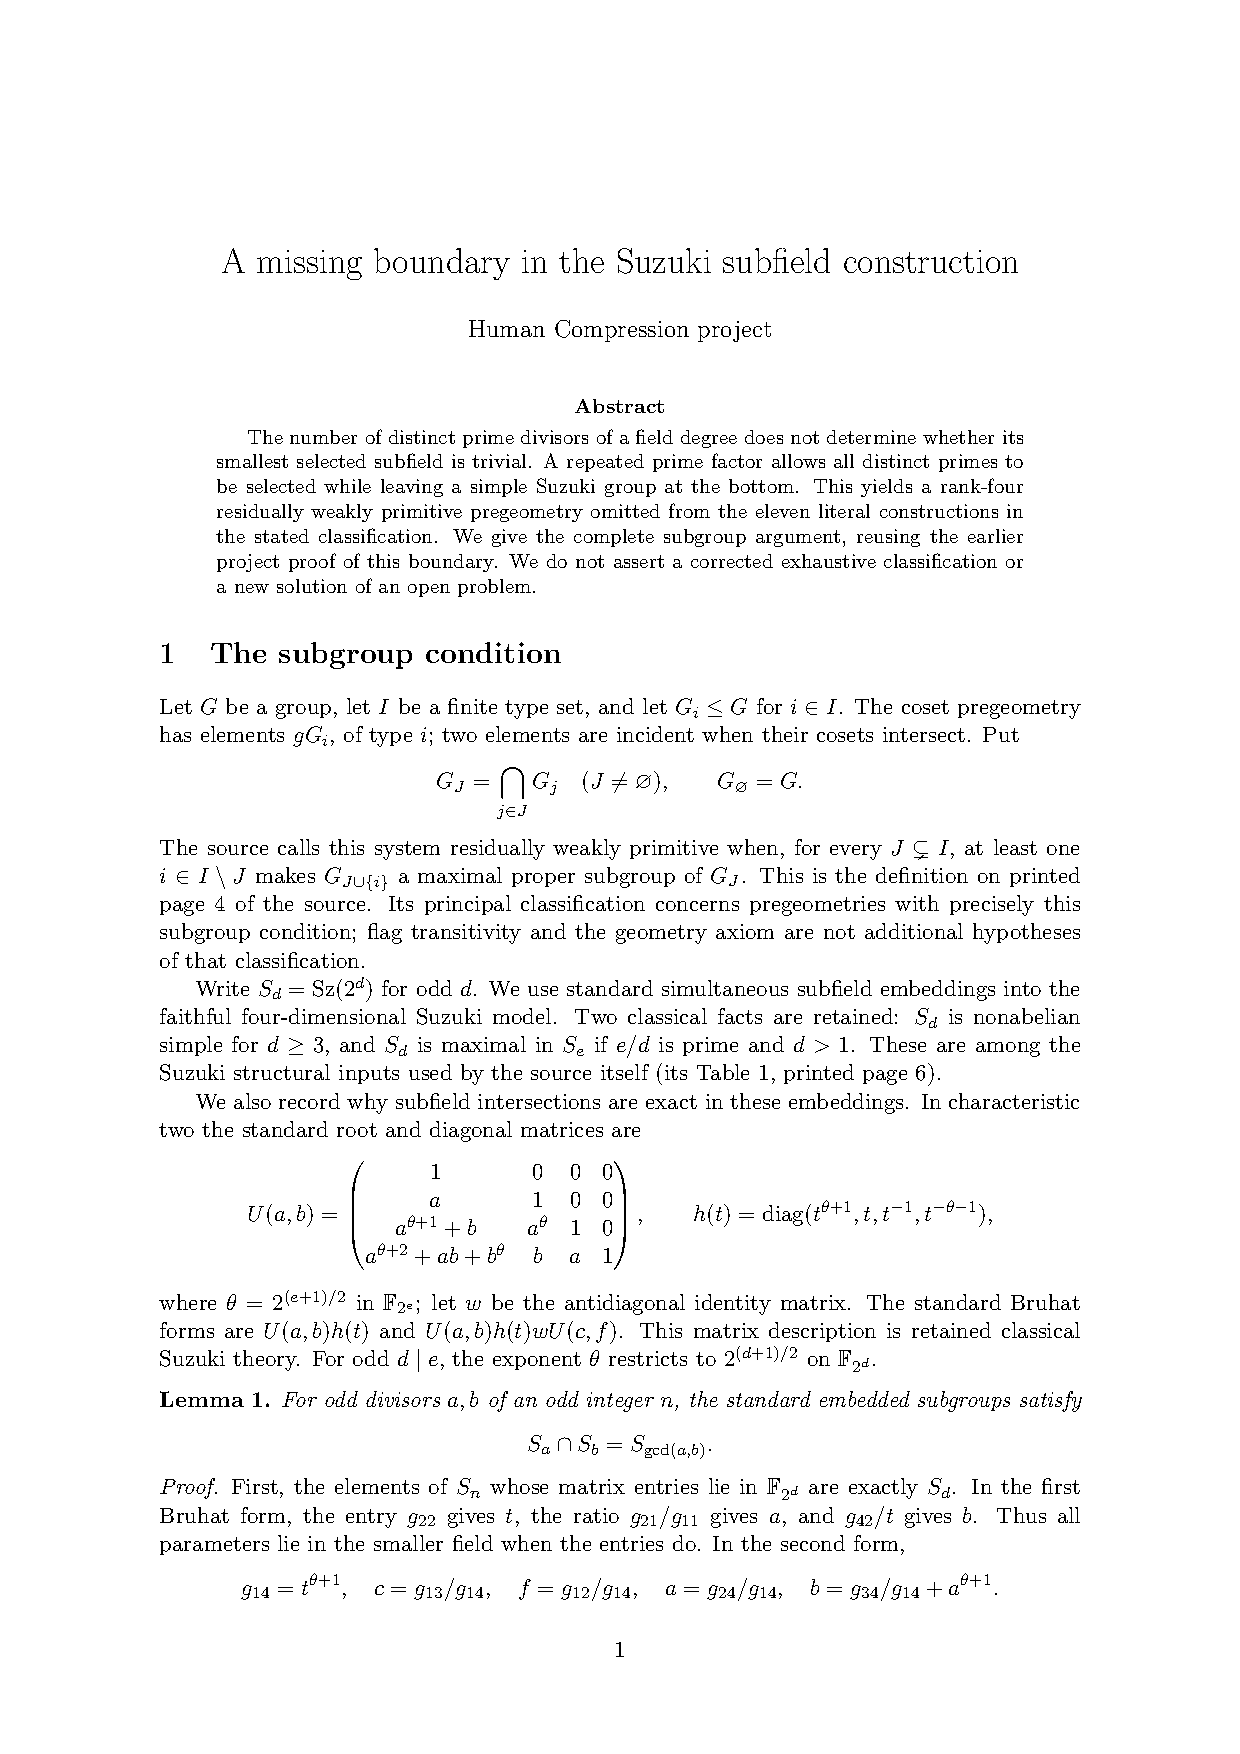
\includepdf[pages=-]{proofs/principal_boundary.pdf}
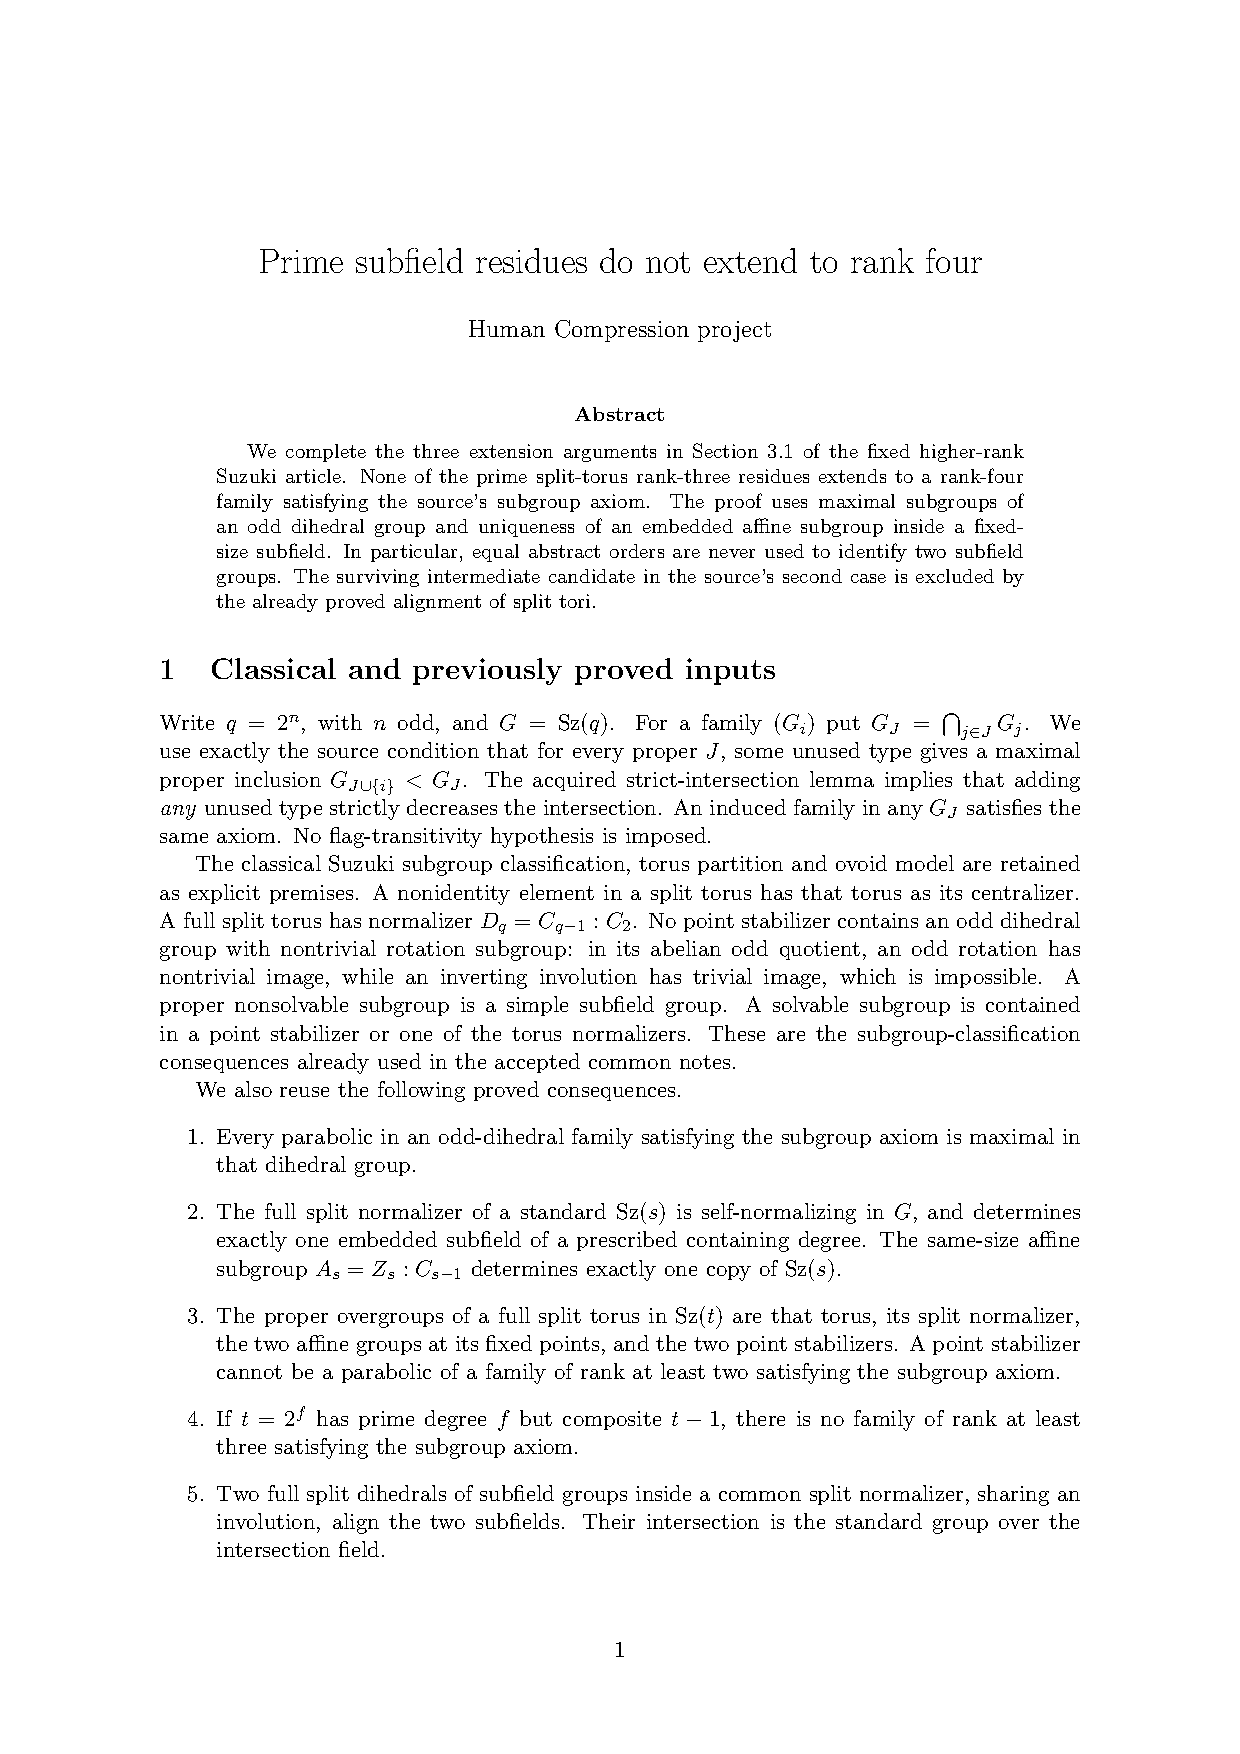
\includepdf[pages=-]{proofs/prime_extensions.pdf}
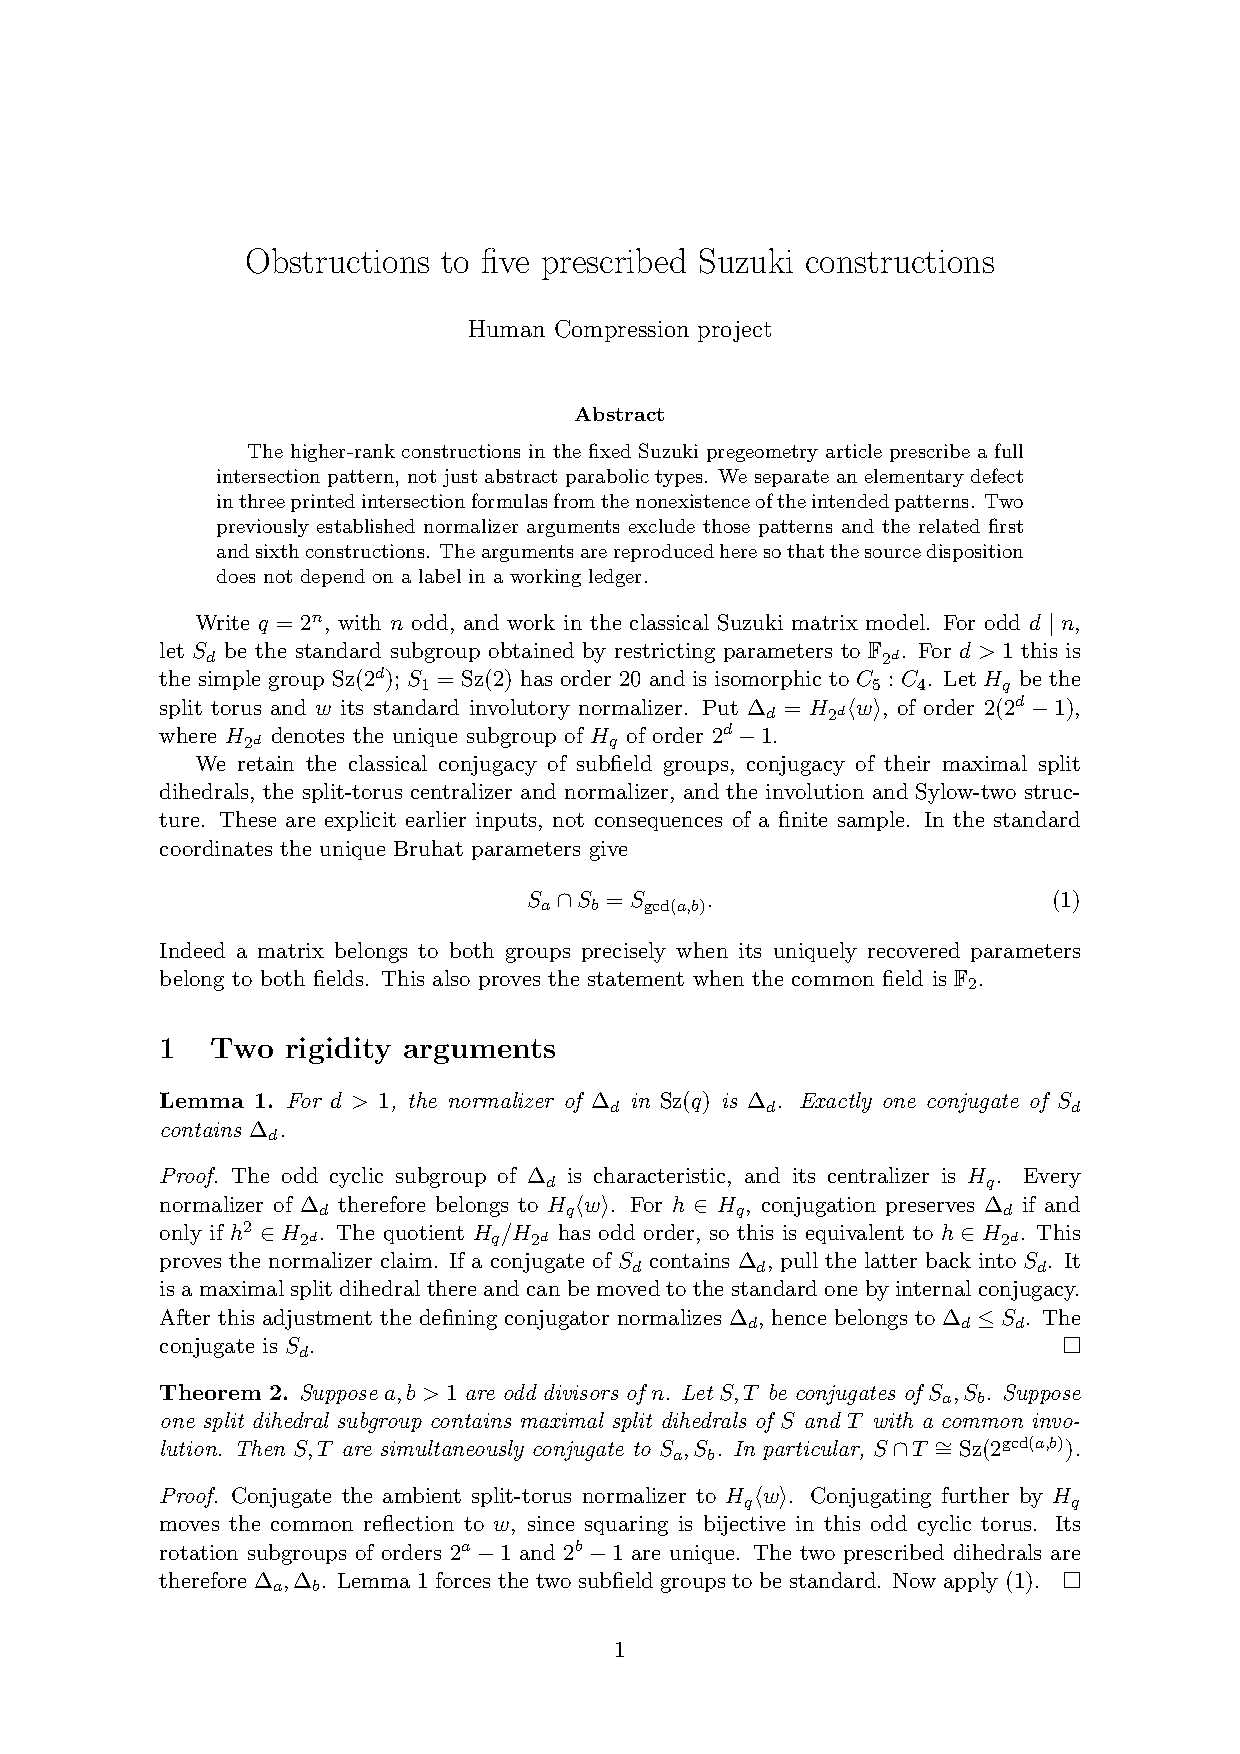
\includepdf[pages=-]{proofs/higher_obstructions.pdf}
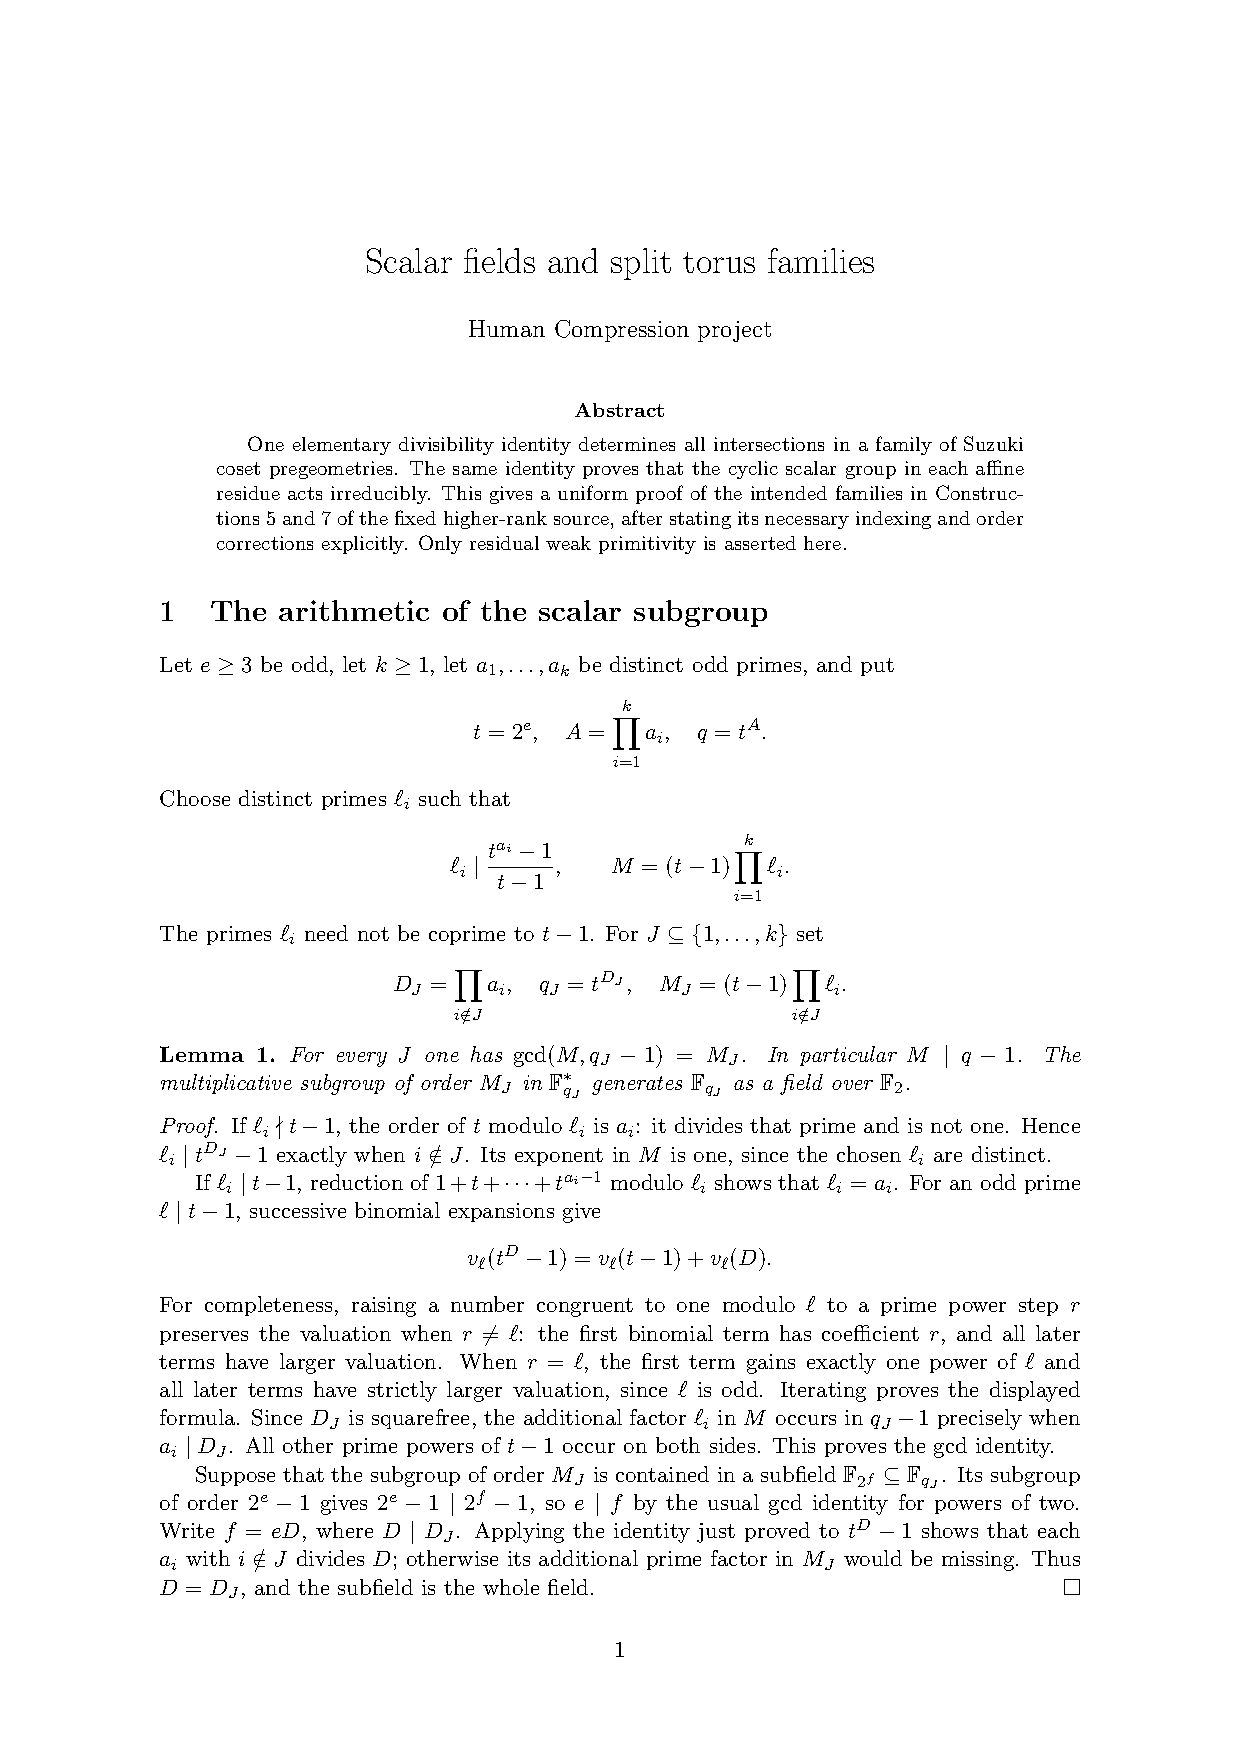
\includepdf[pages=-]{proofs/split_families.pdf}
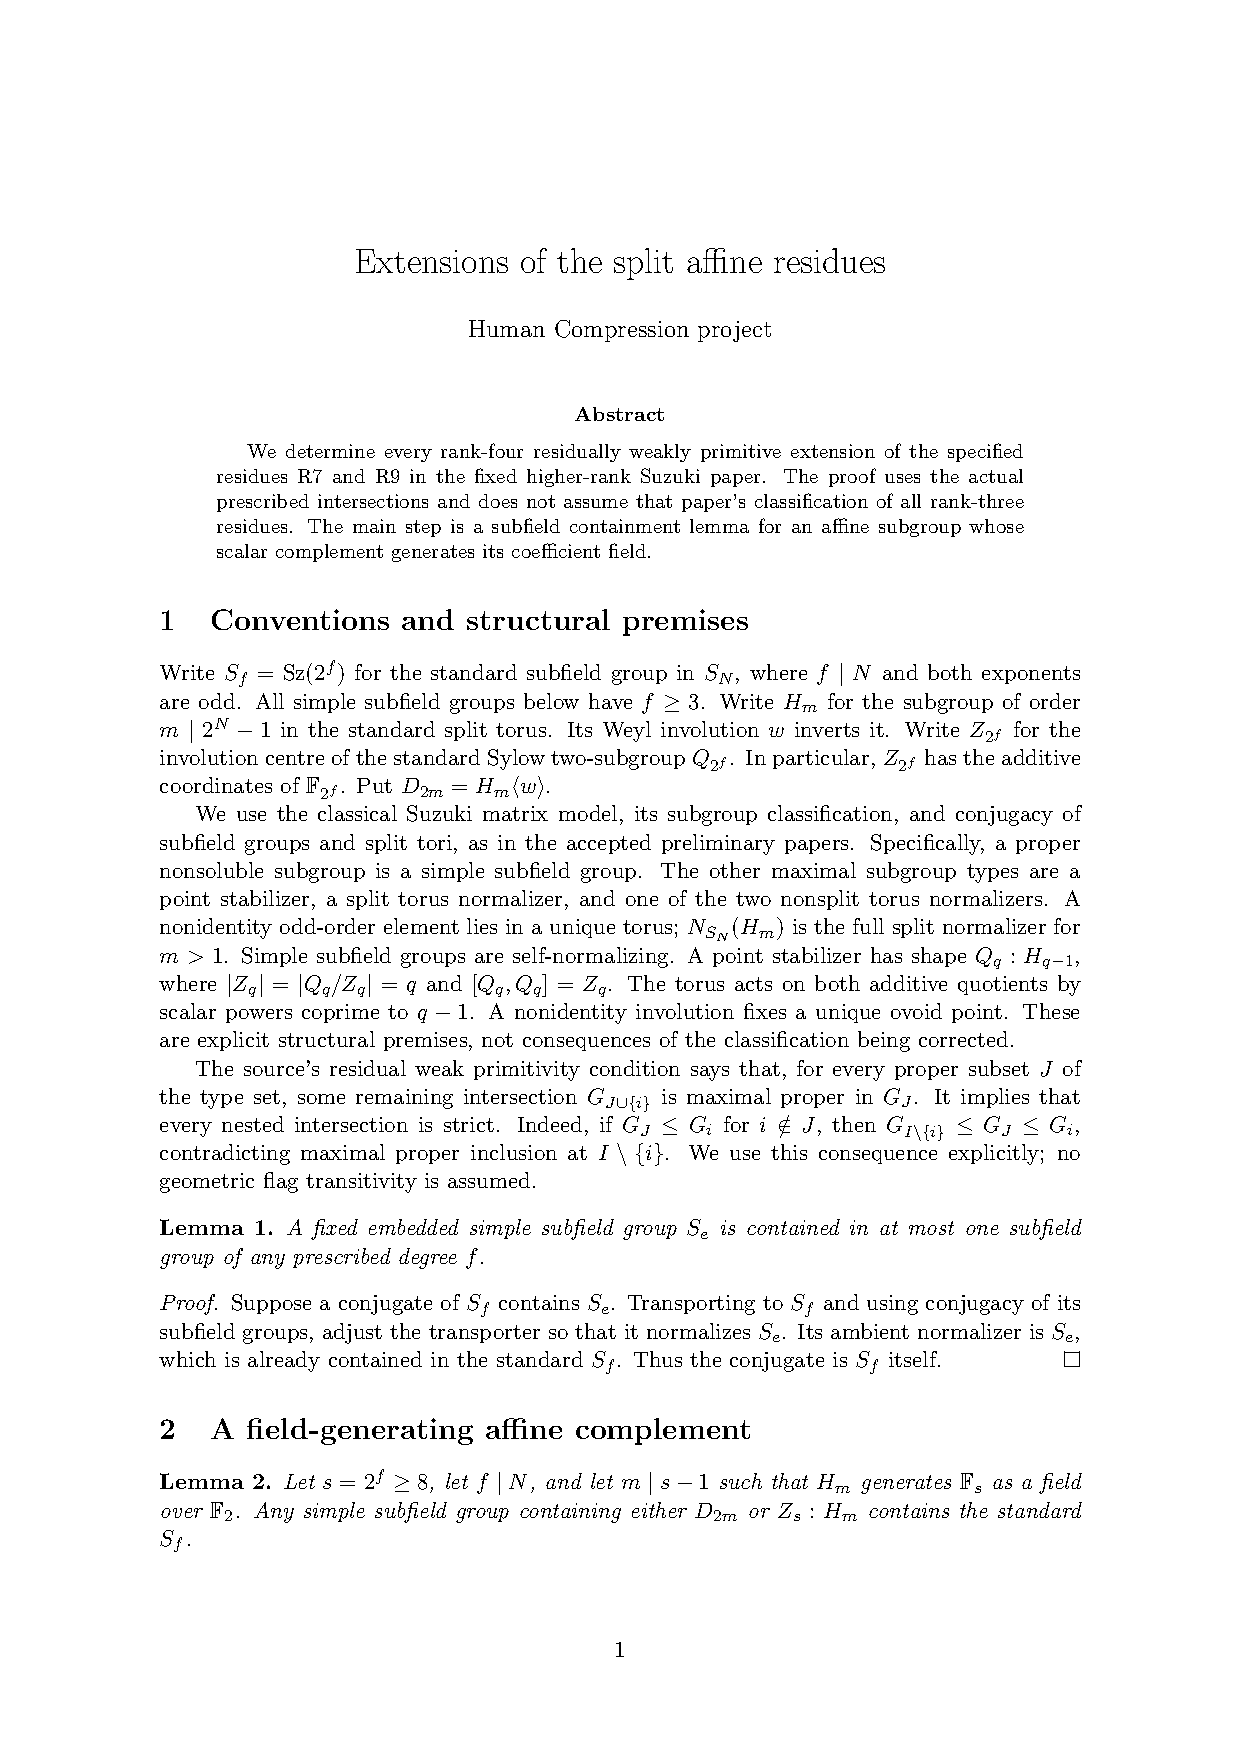
\includepdf[pages=-]{proofs/split_necessity.pdf}
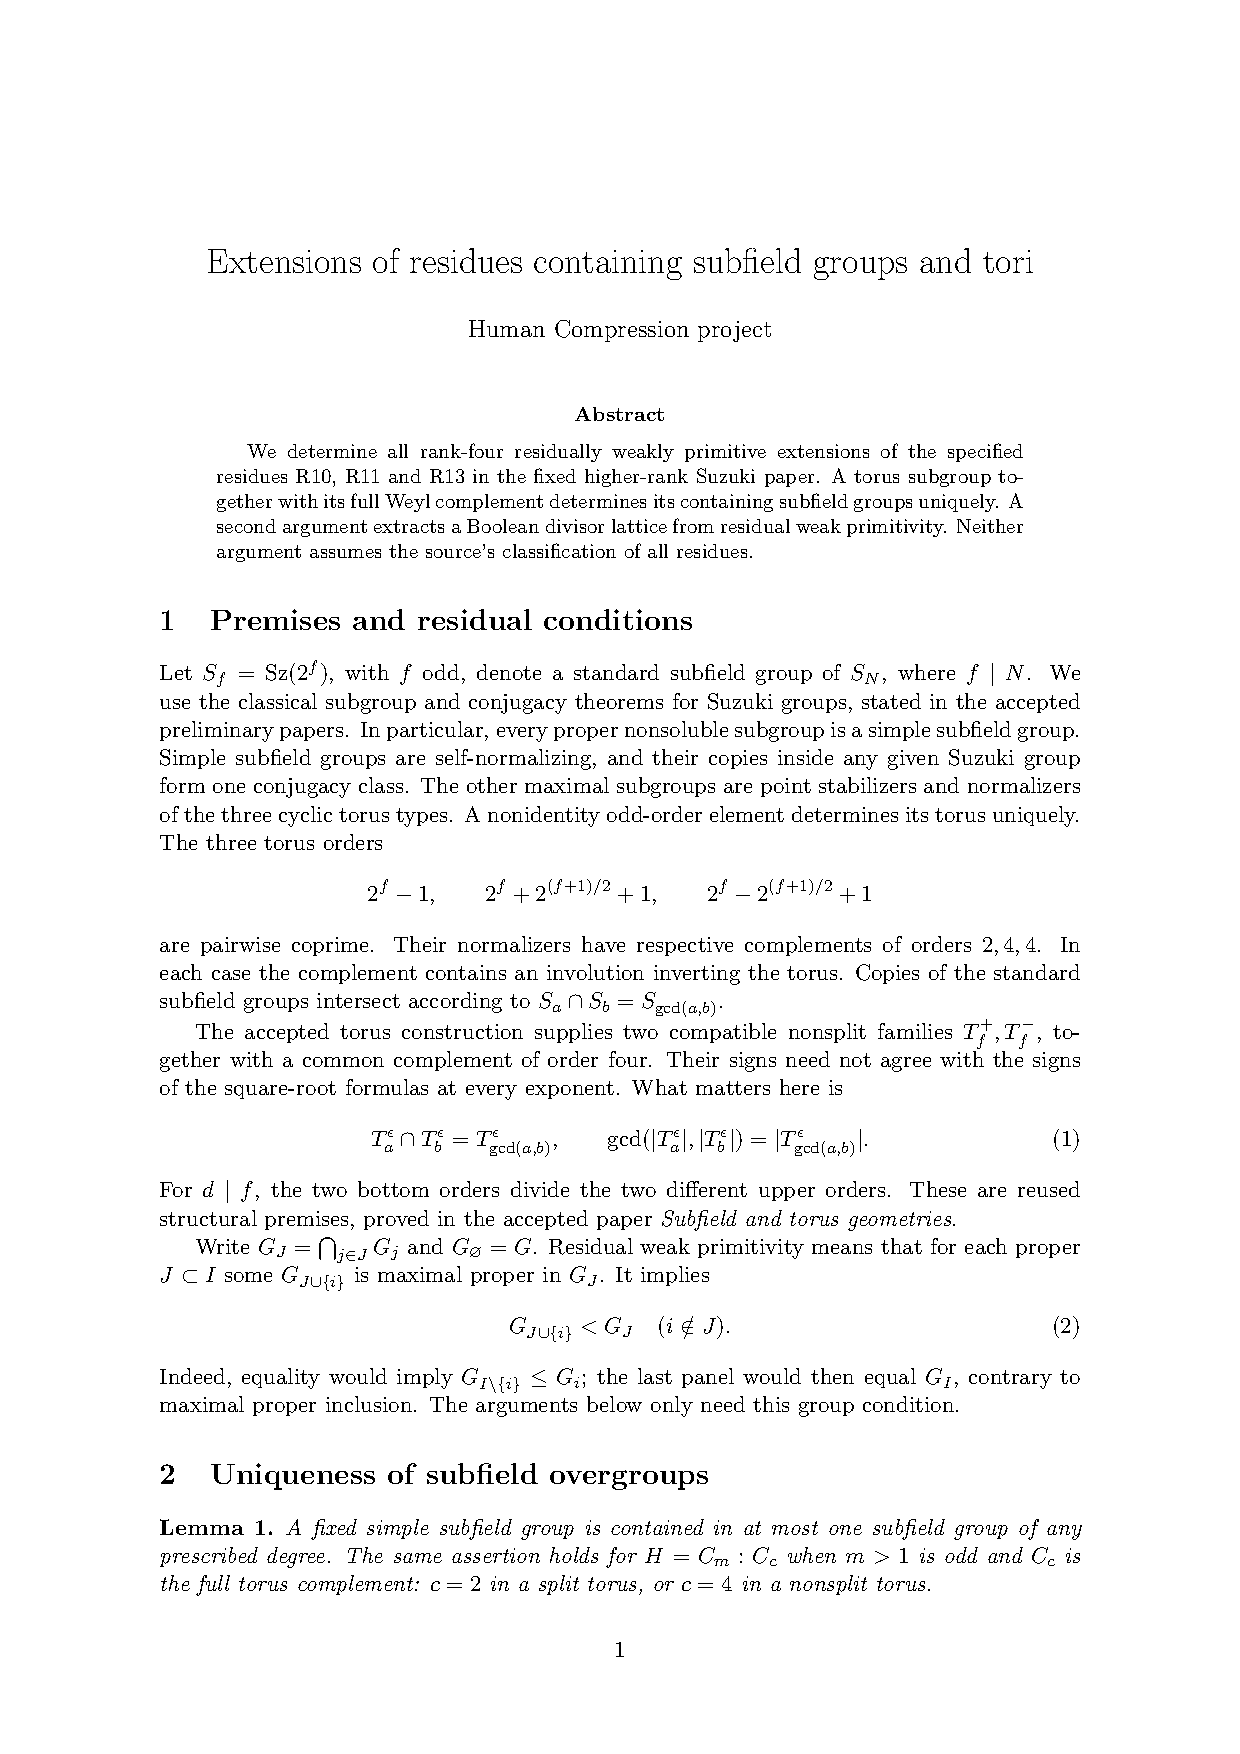
\includepdf[pages=-]{proofs/torus_necessity.pdf}
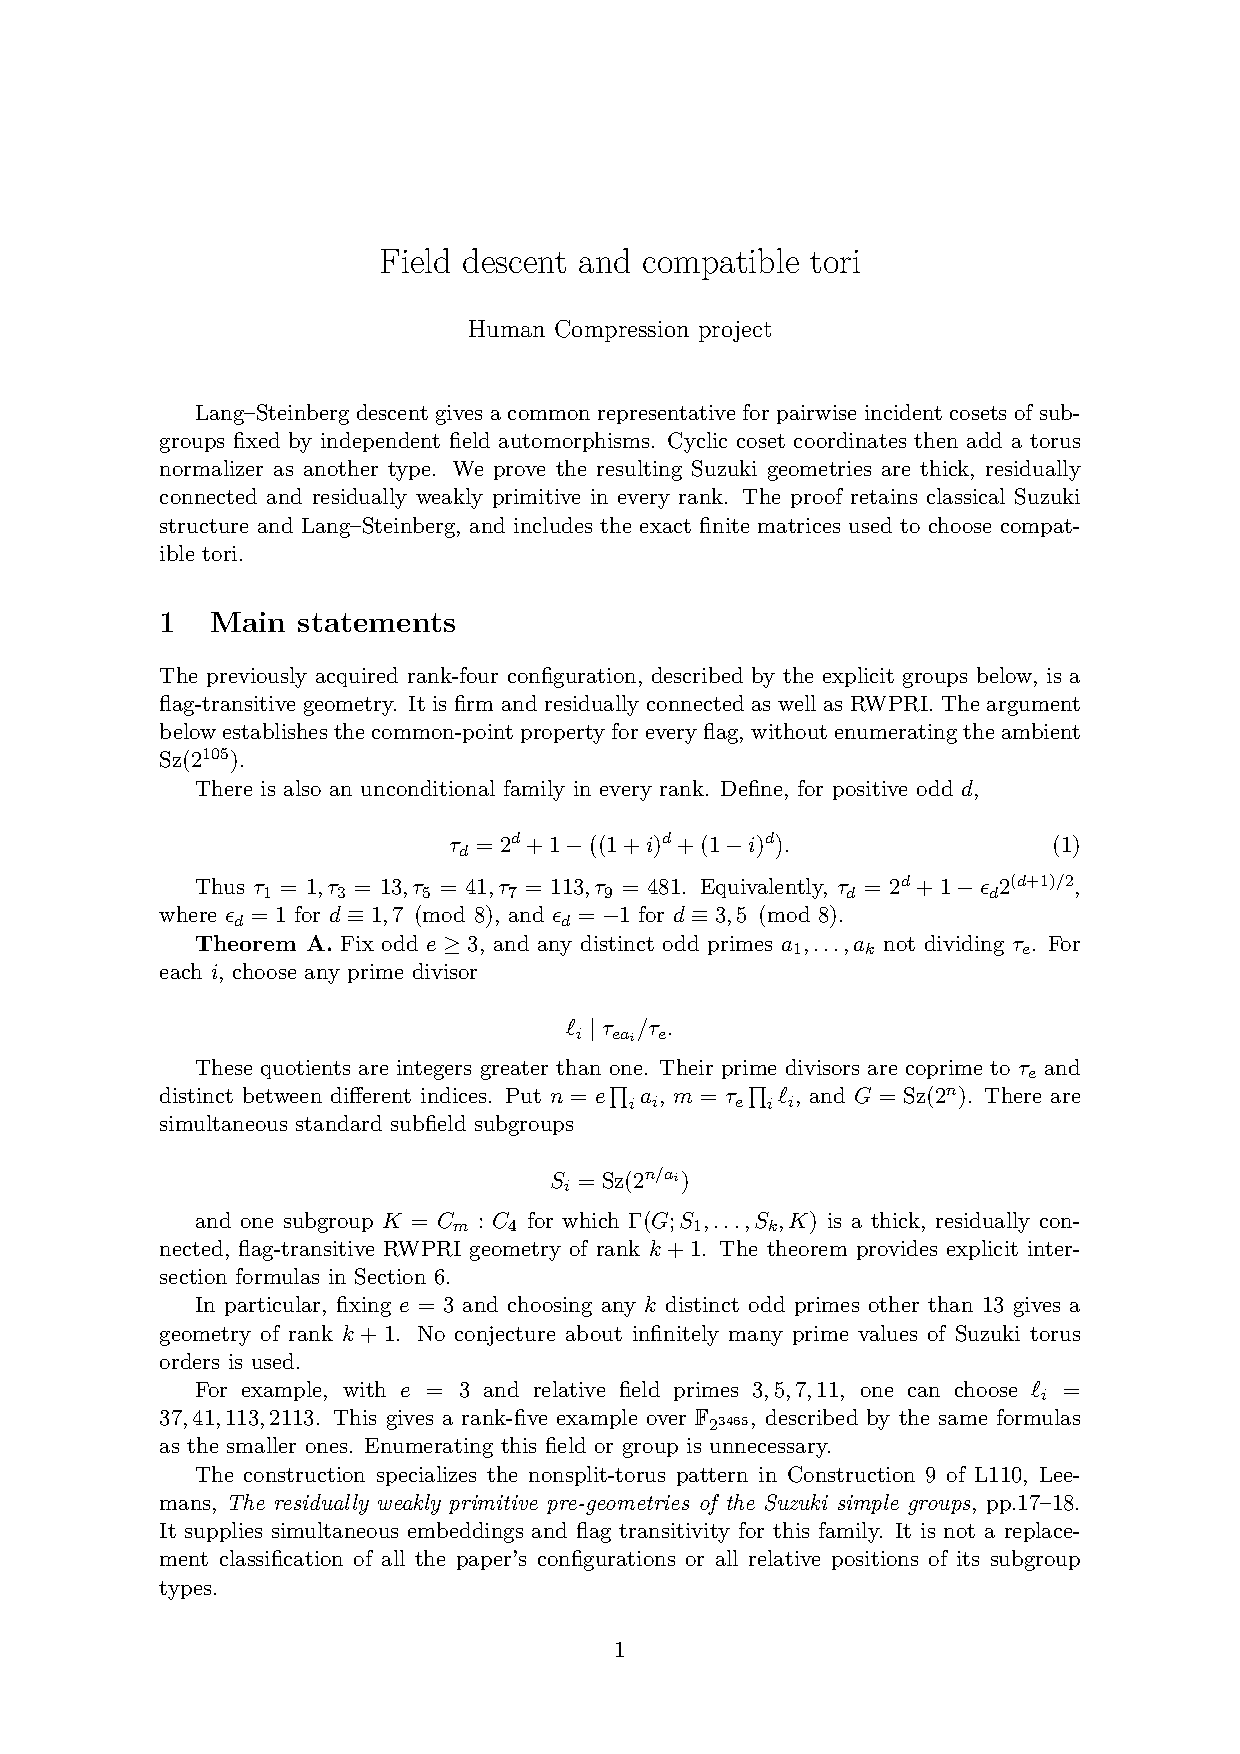
\includepdf[pages=-]{proofs/descent.pdf}
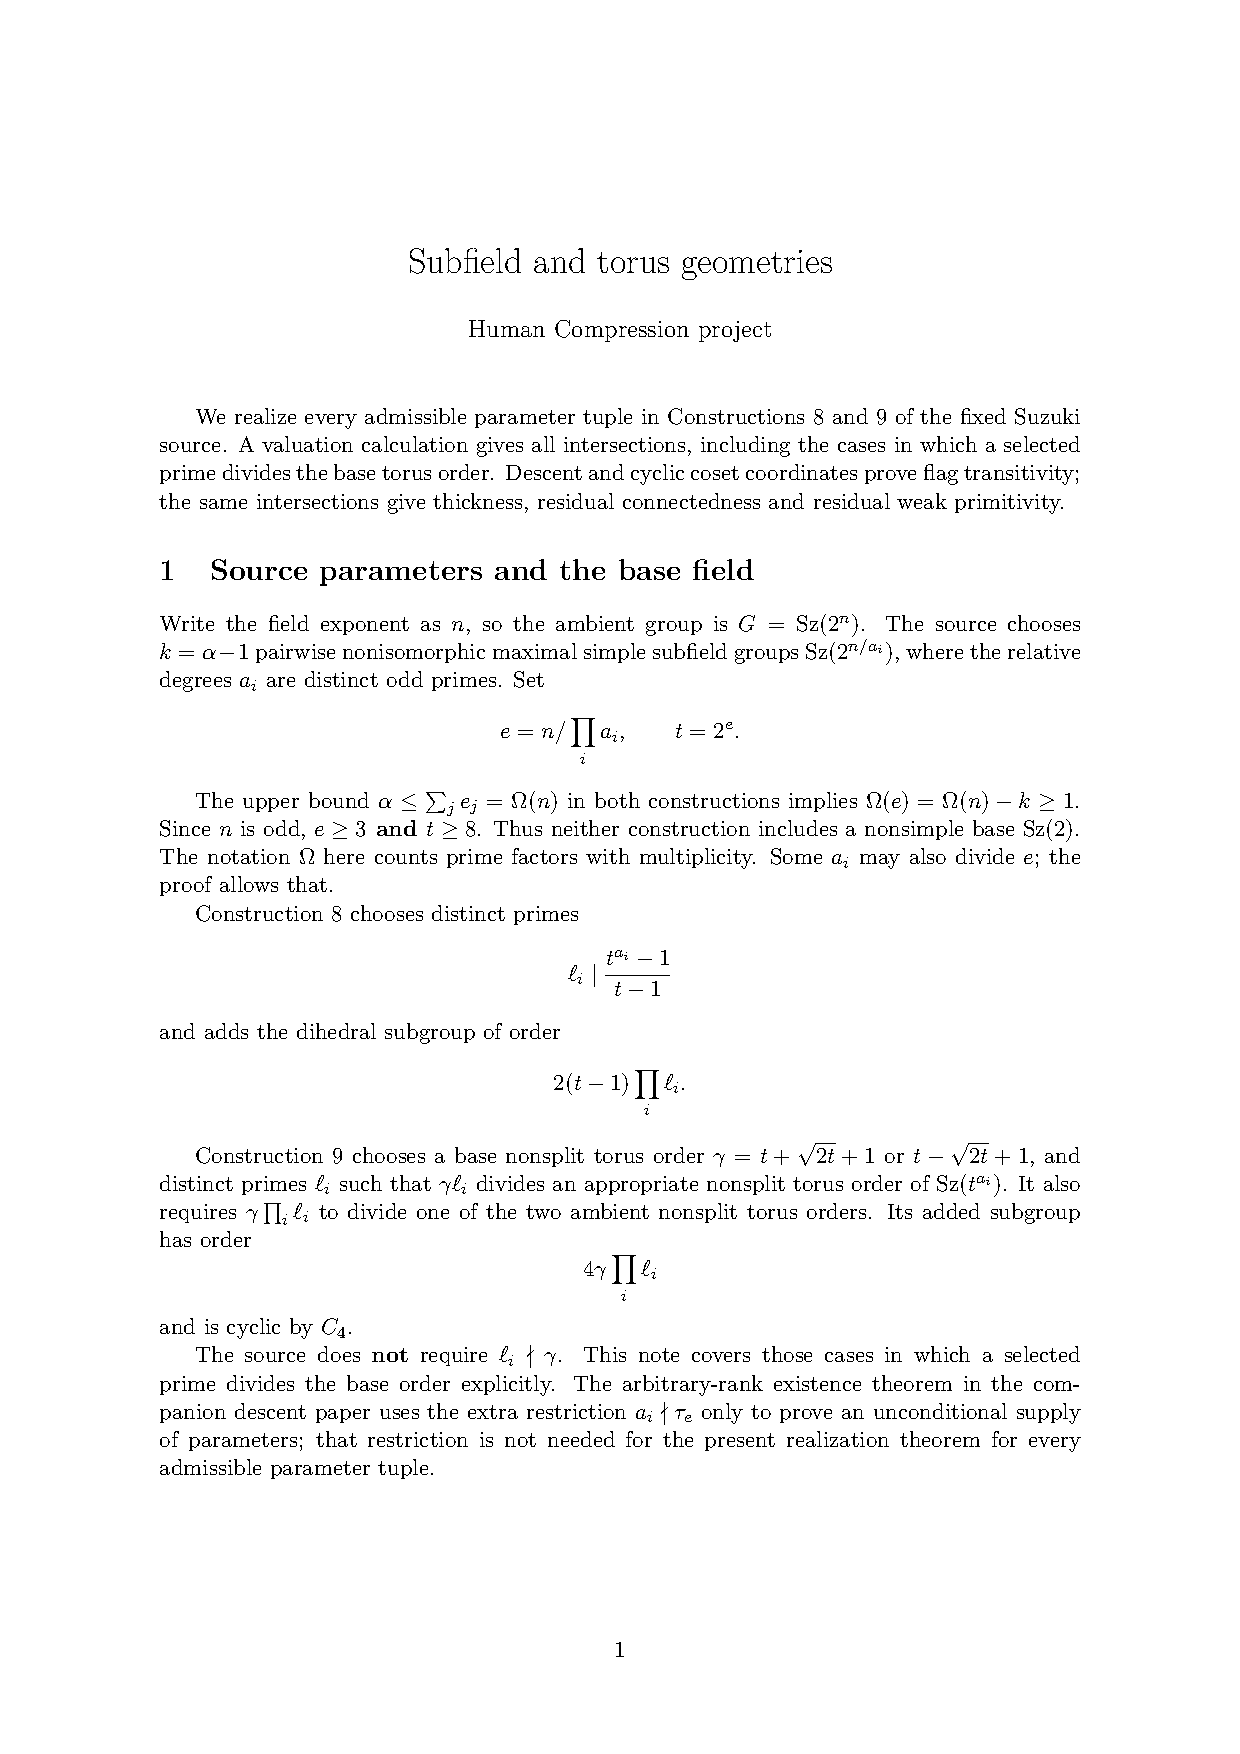
\includepdf[pages=-]{proofs/torus_families.pdf}
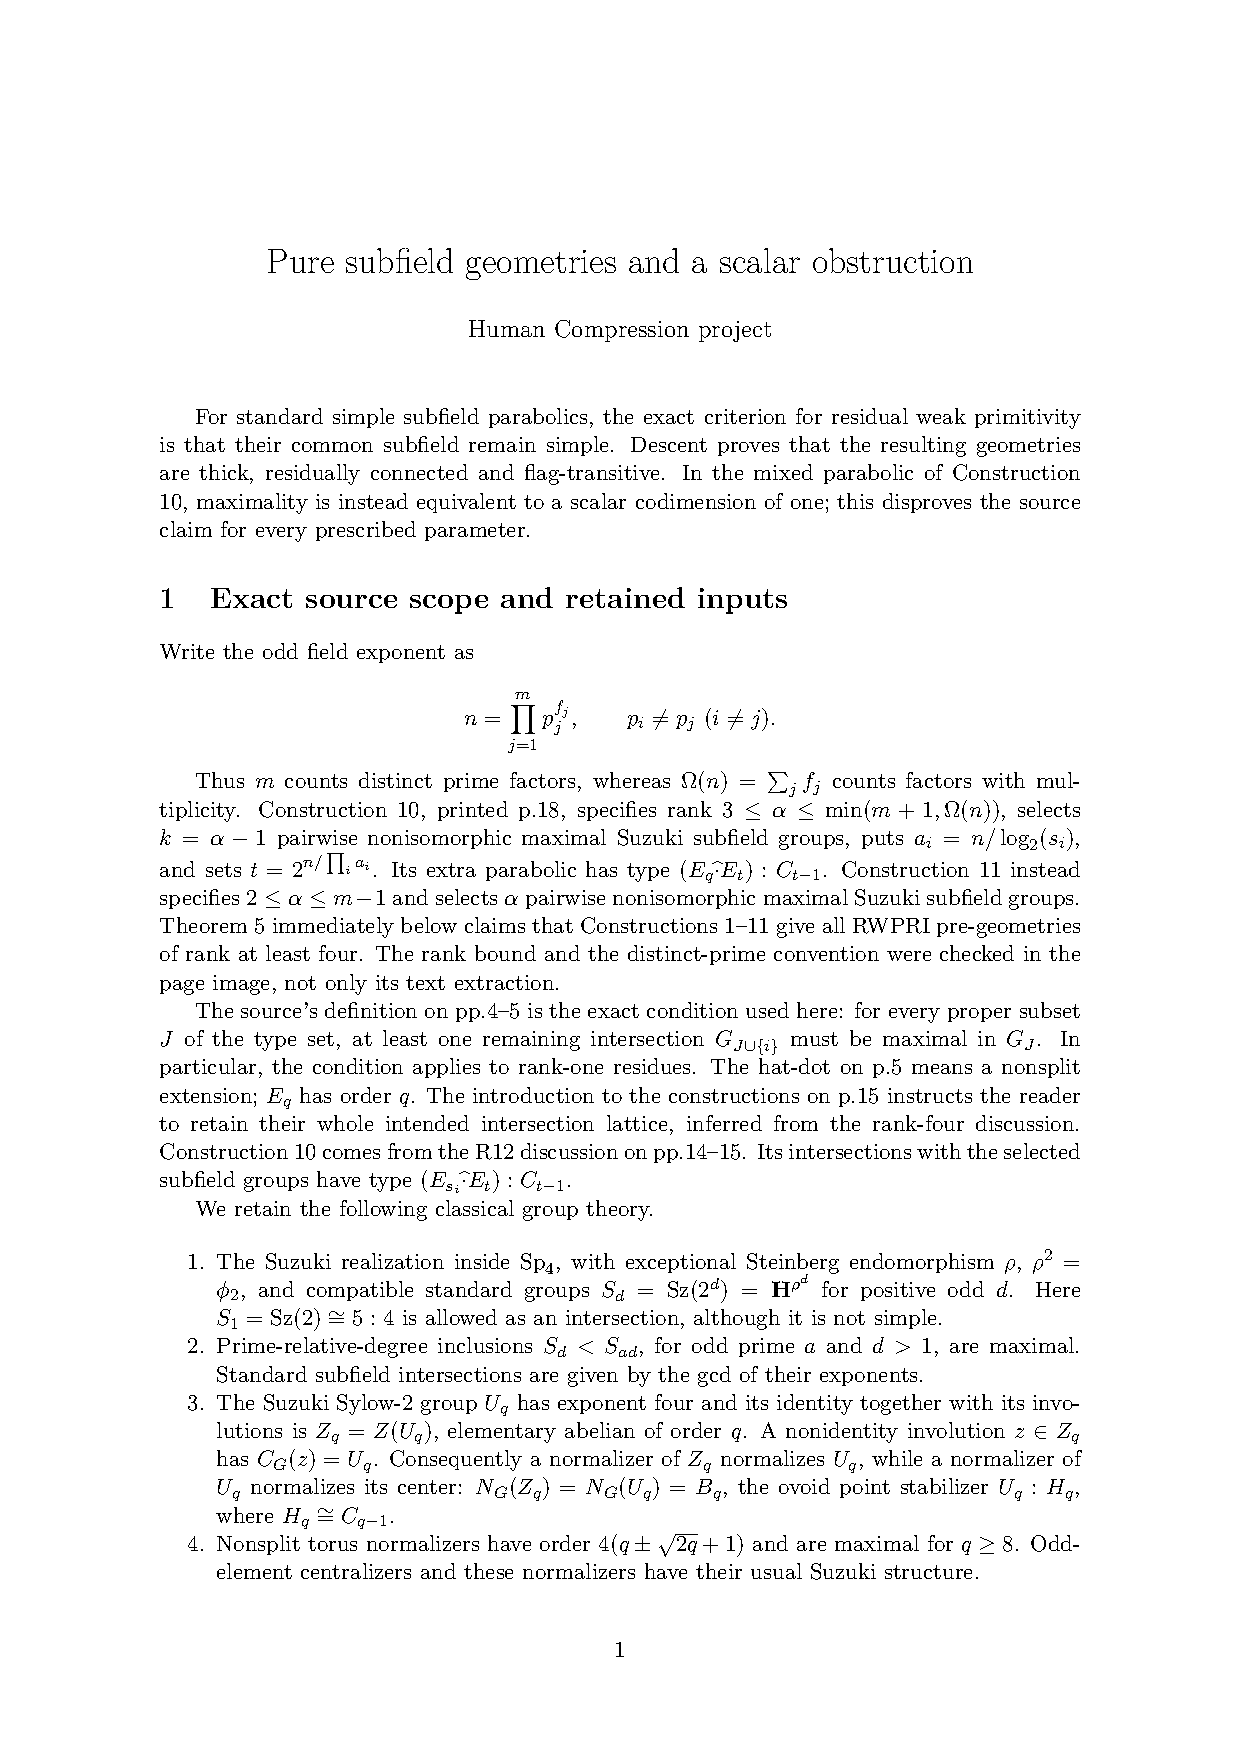
\includepdf[pages=-]{proofs/pure_mixed.pdf}
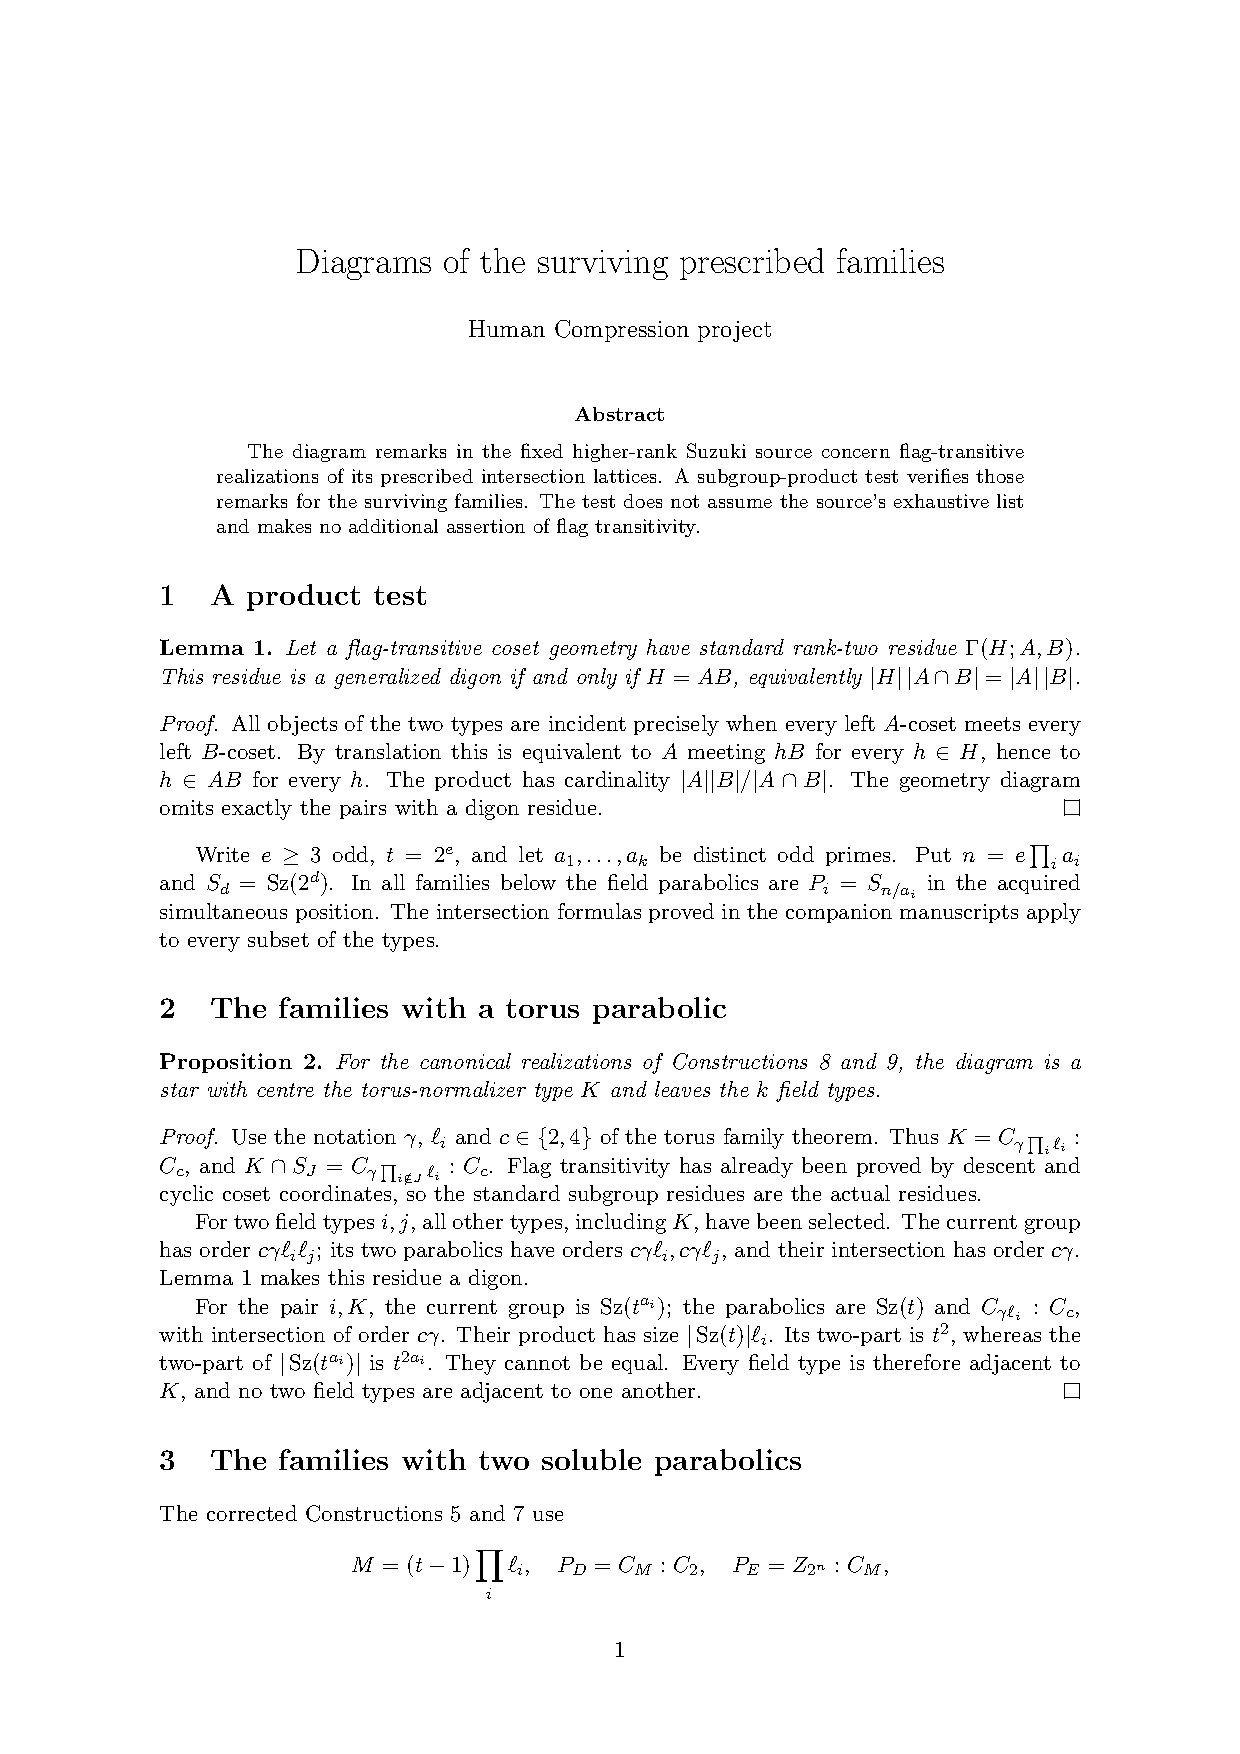
\includepdf[pages=-]{proofs/diagrams.pdf}
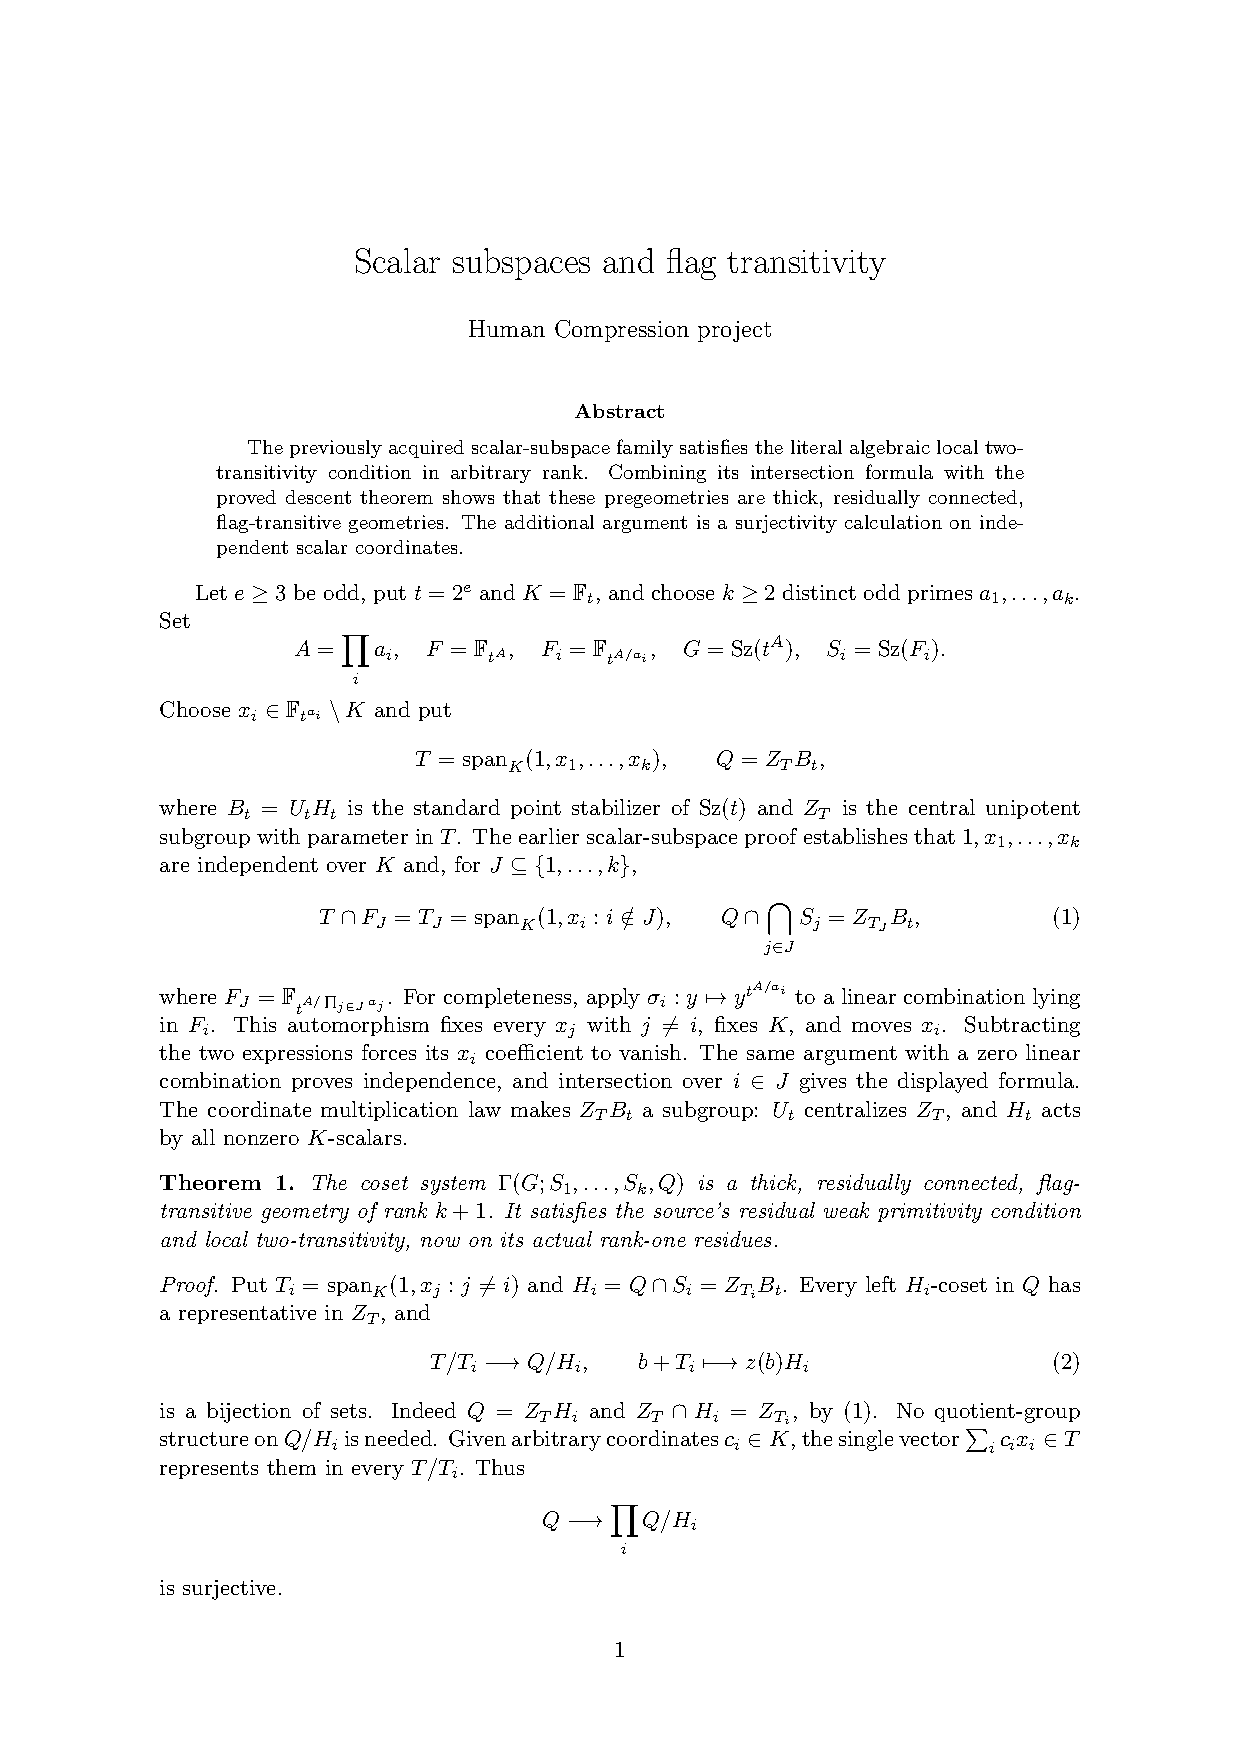
\includepdf[pages=-]{proofs/local_geometry.pdf}
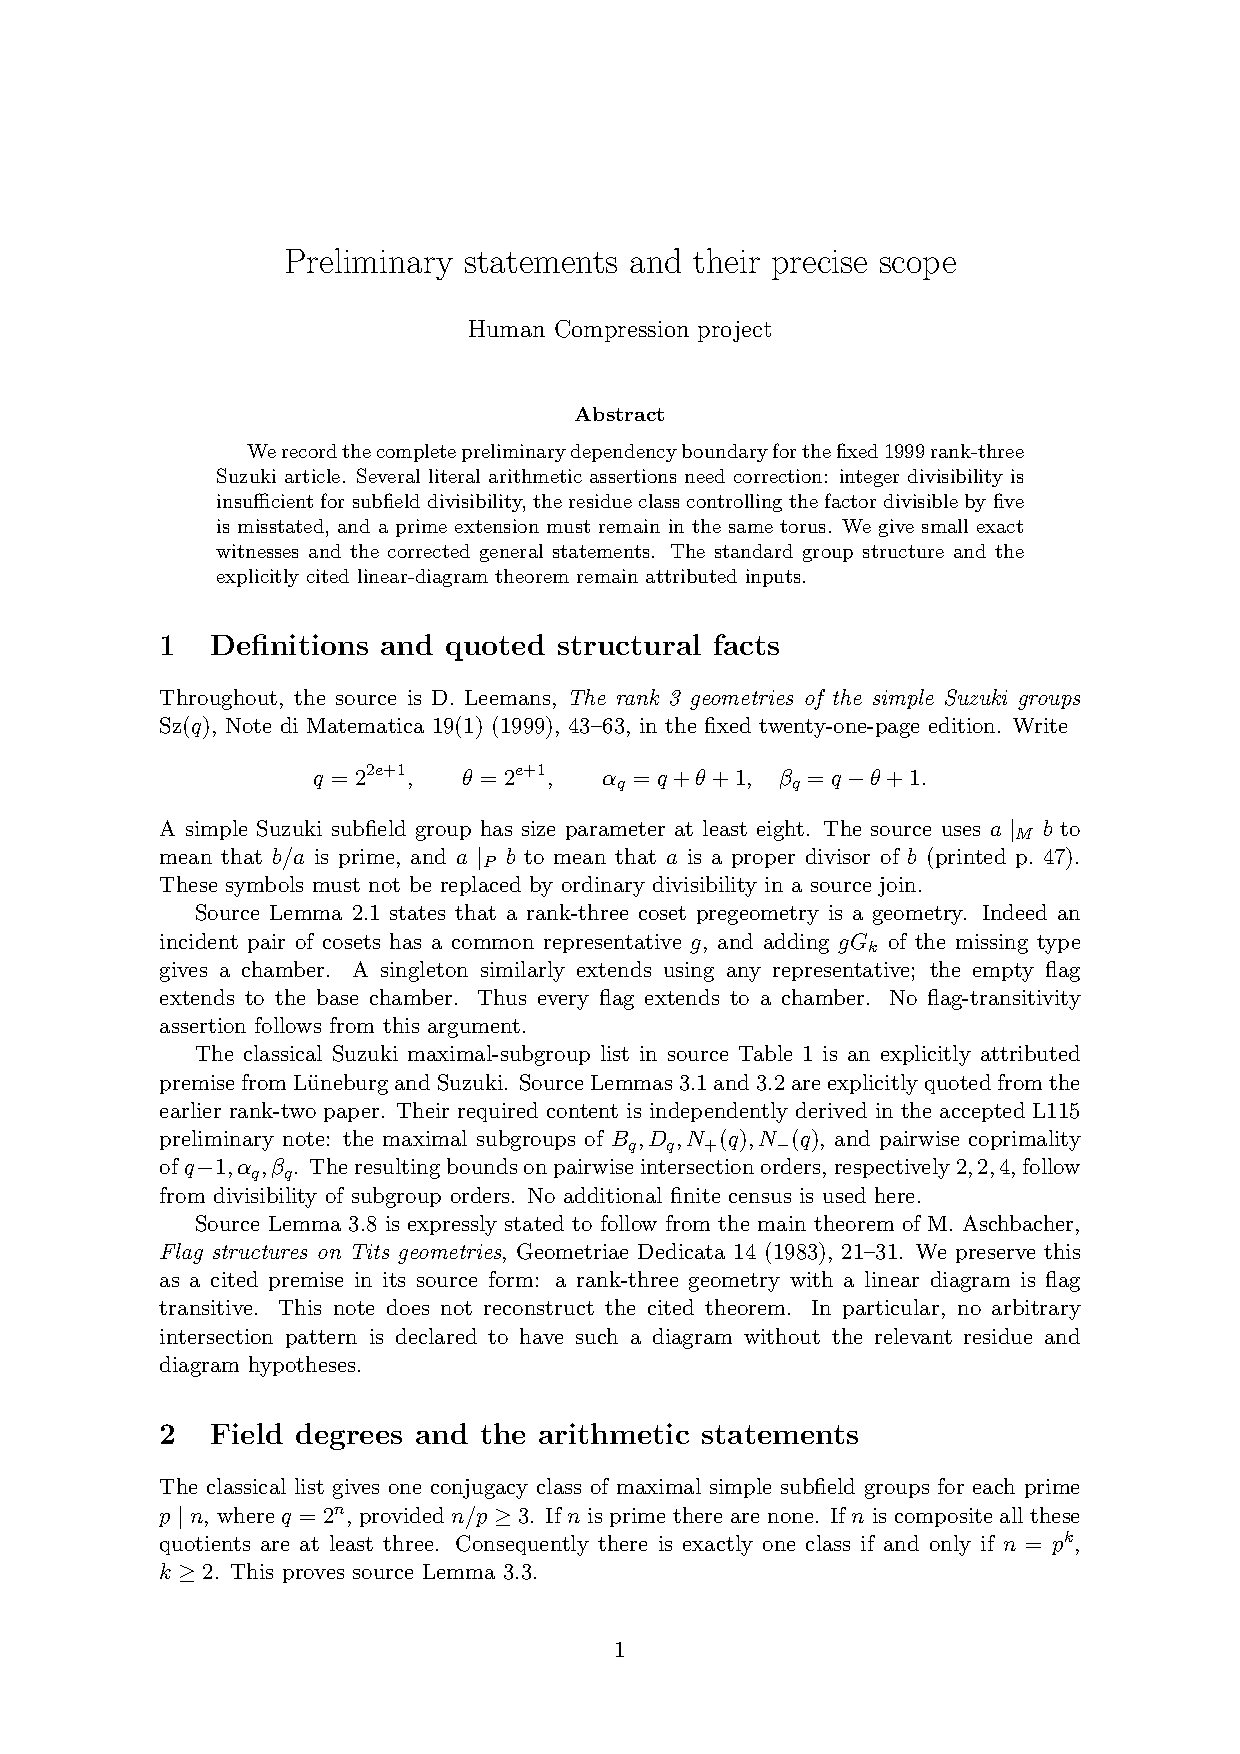
\includepdf[pages=-]{proofs/preliminary.pdf}
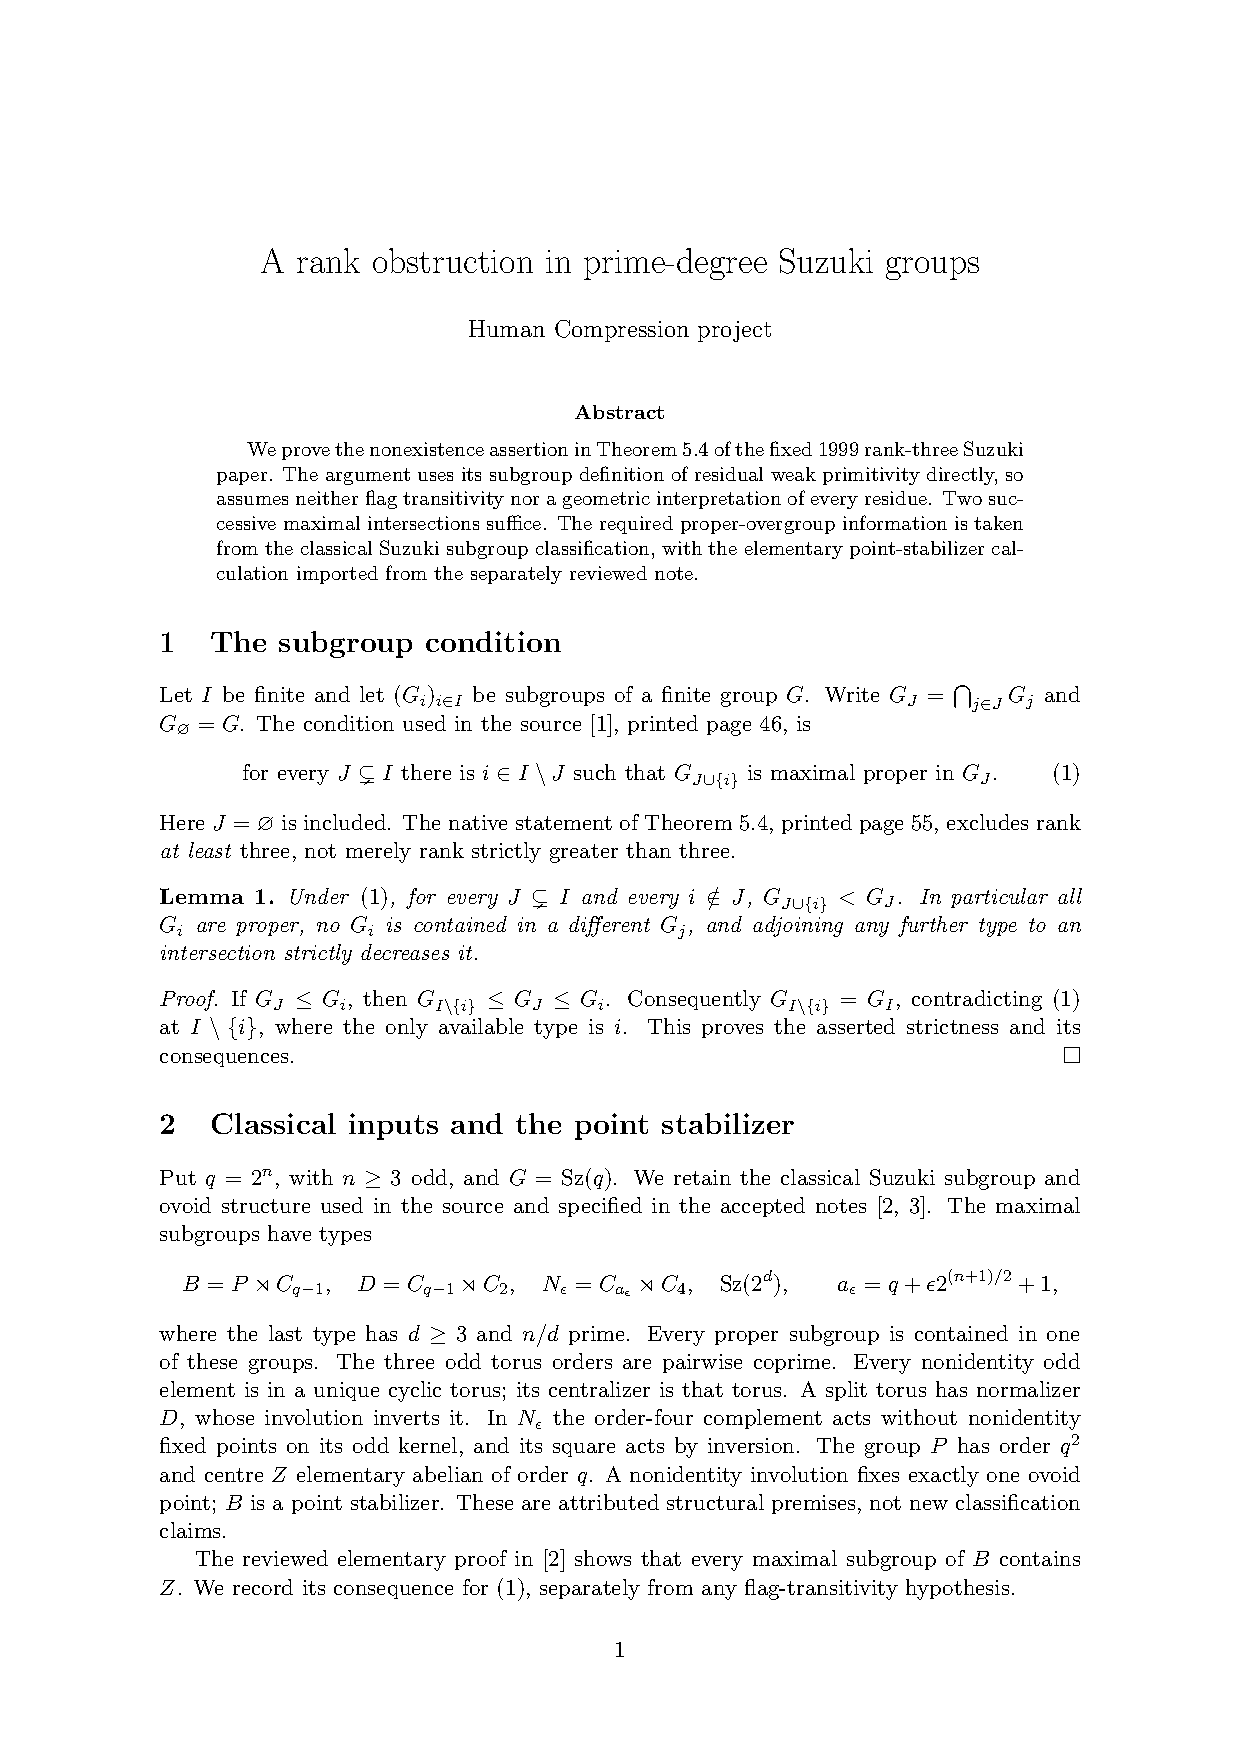
\includepdf[pages=-]{proofs/prime_degree.pdf}
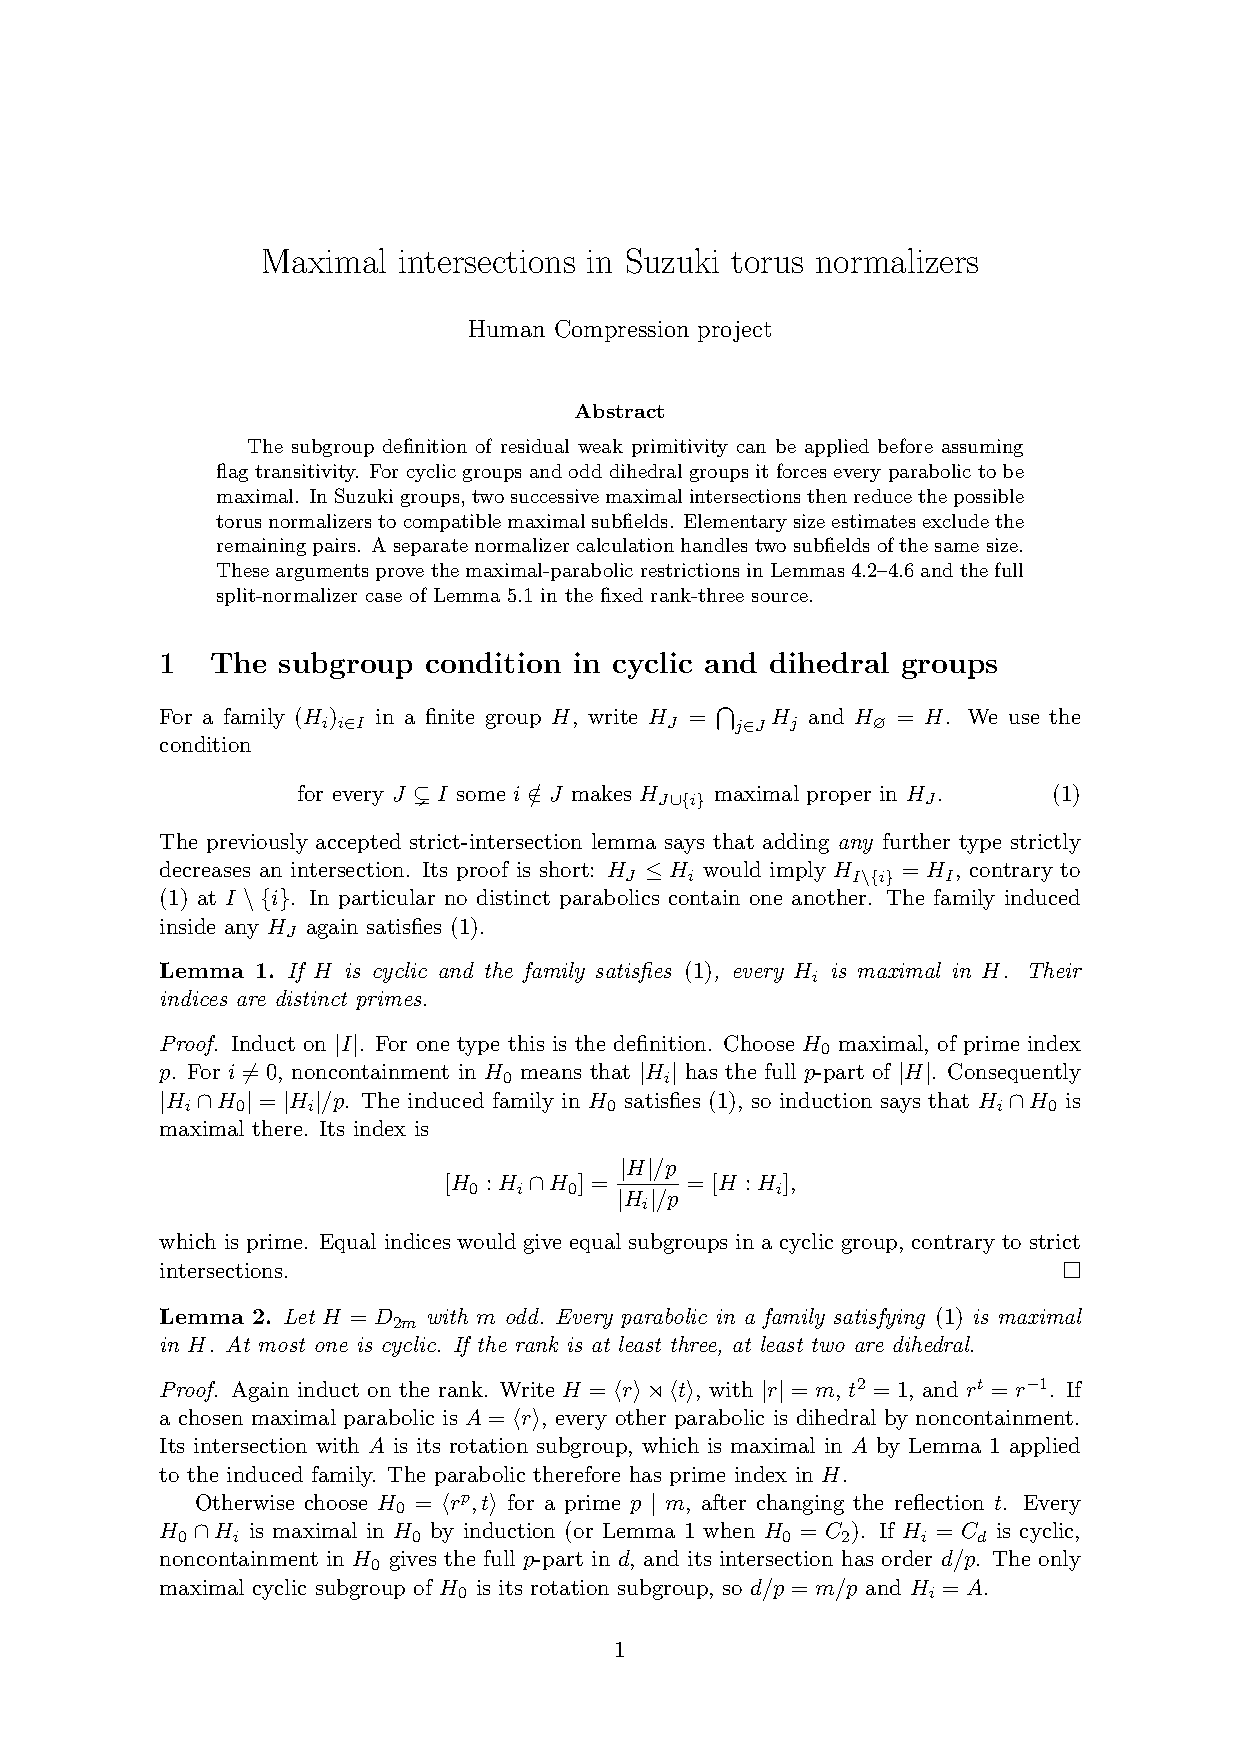
\includepdf[pages=-]{proofs/restrictions.pdf}
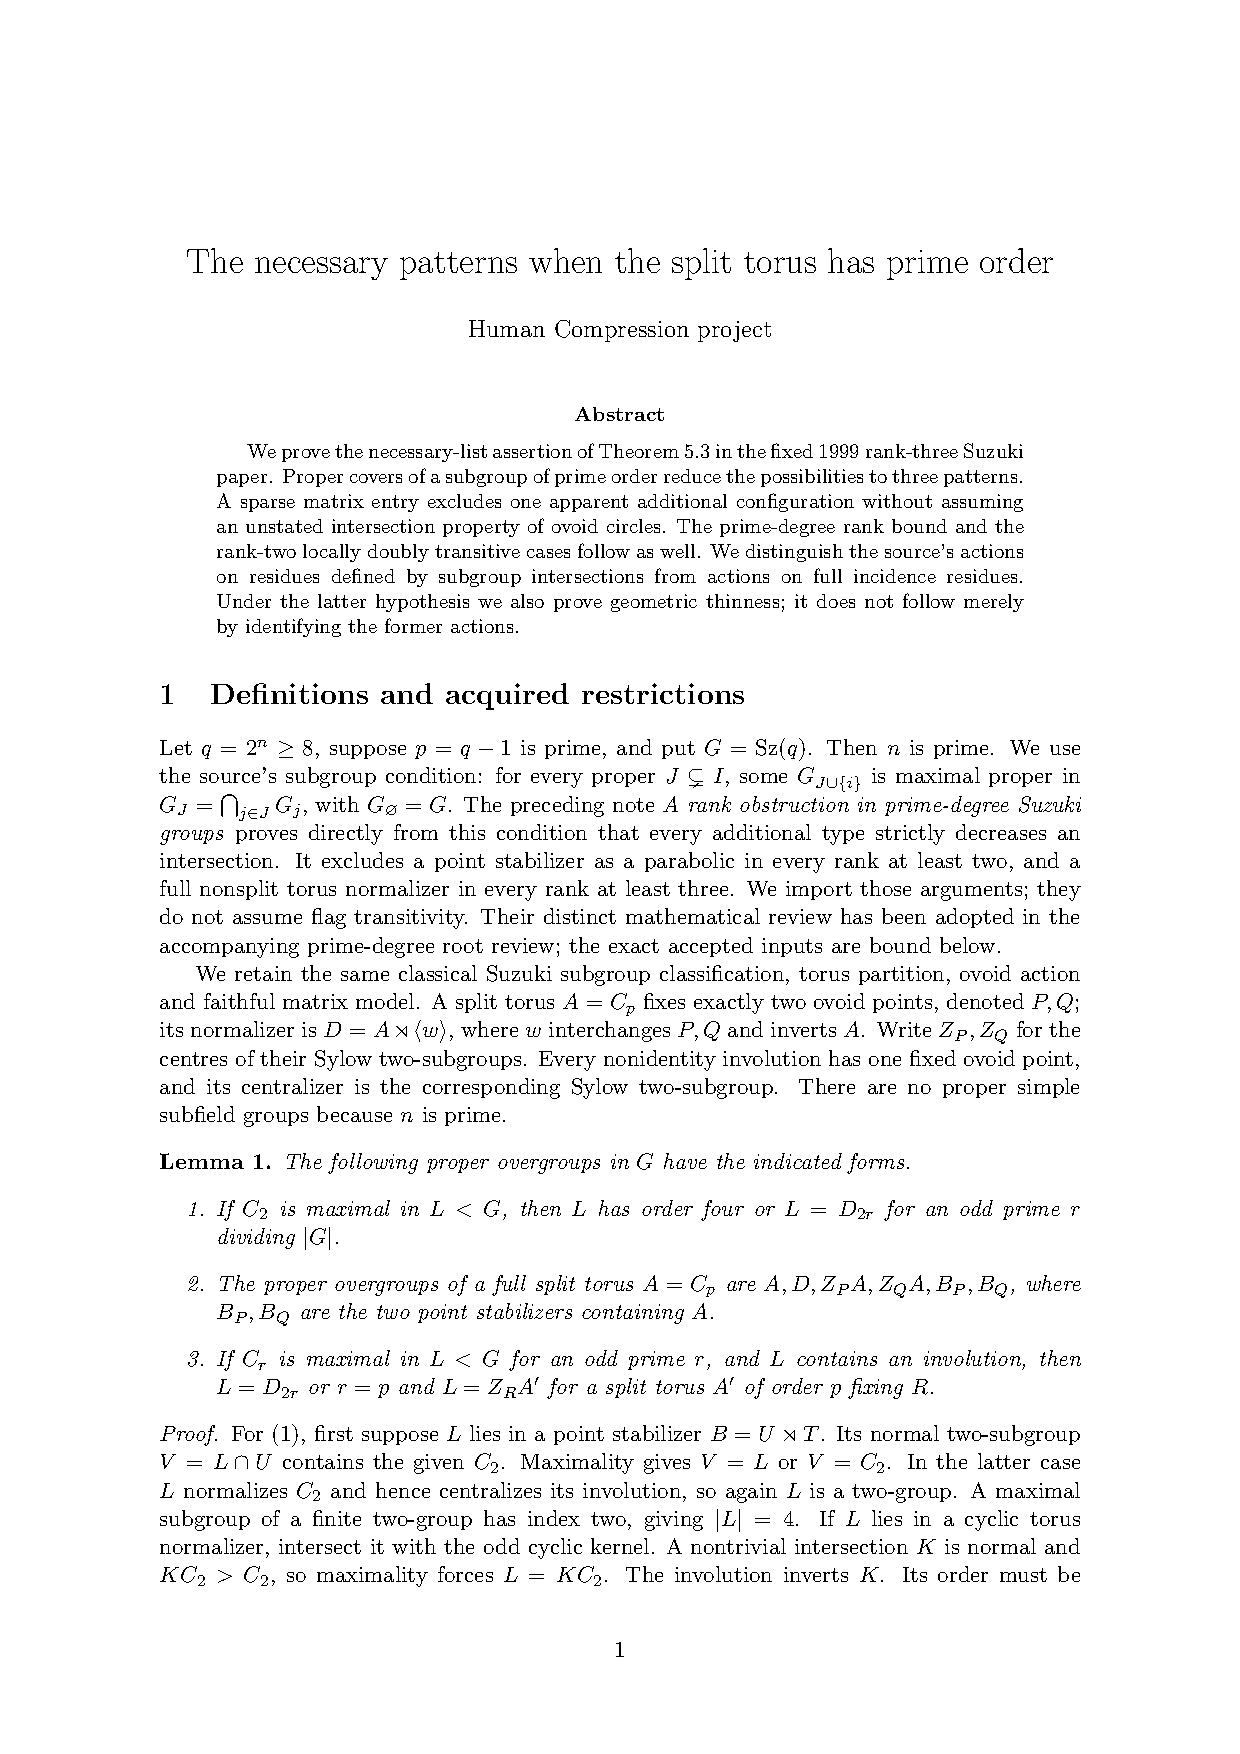
\includepdf[pages=-]{proofs/patterns.pdf}
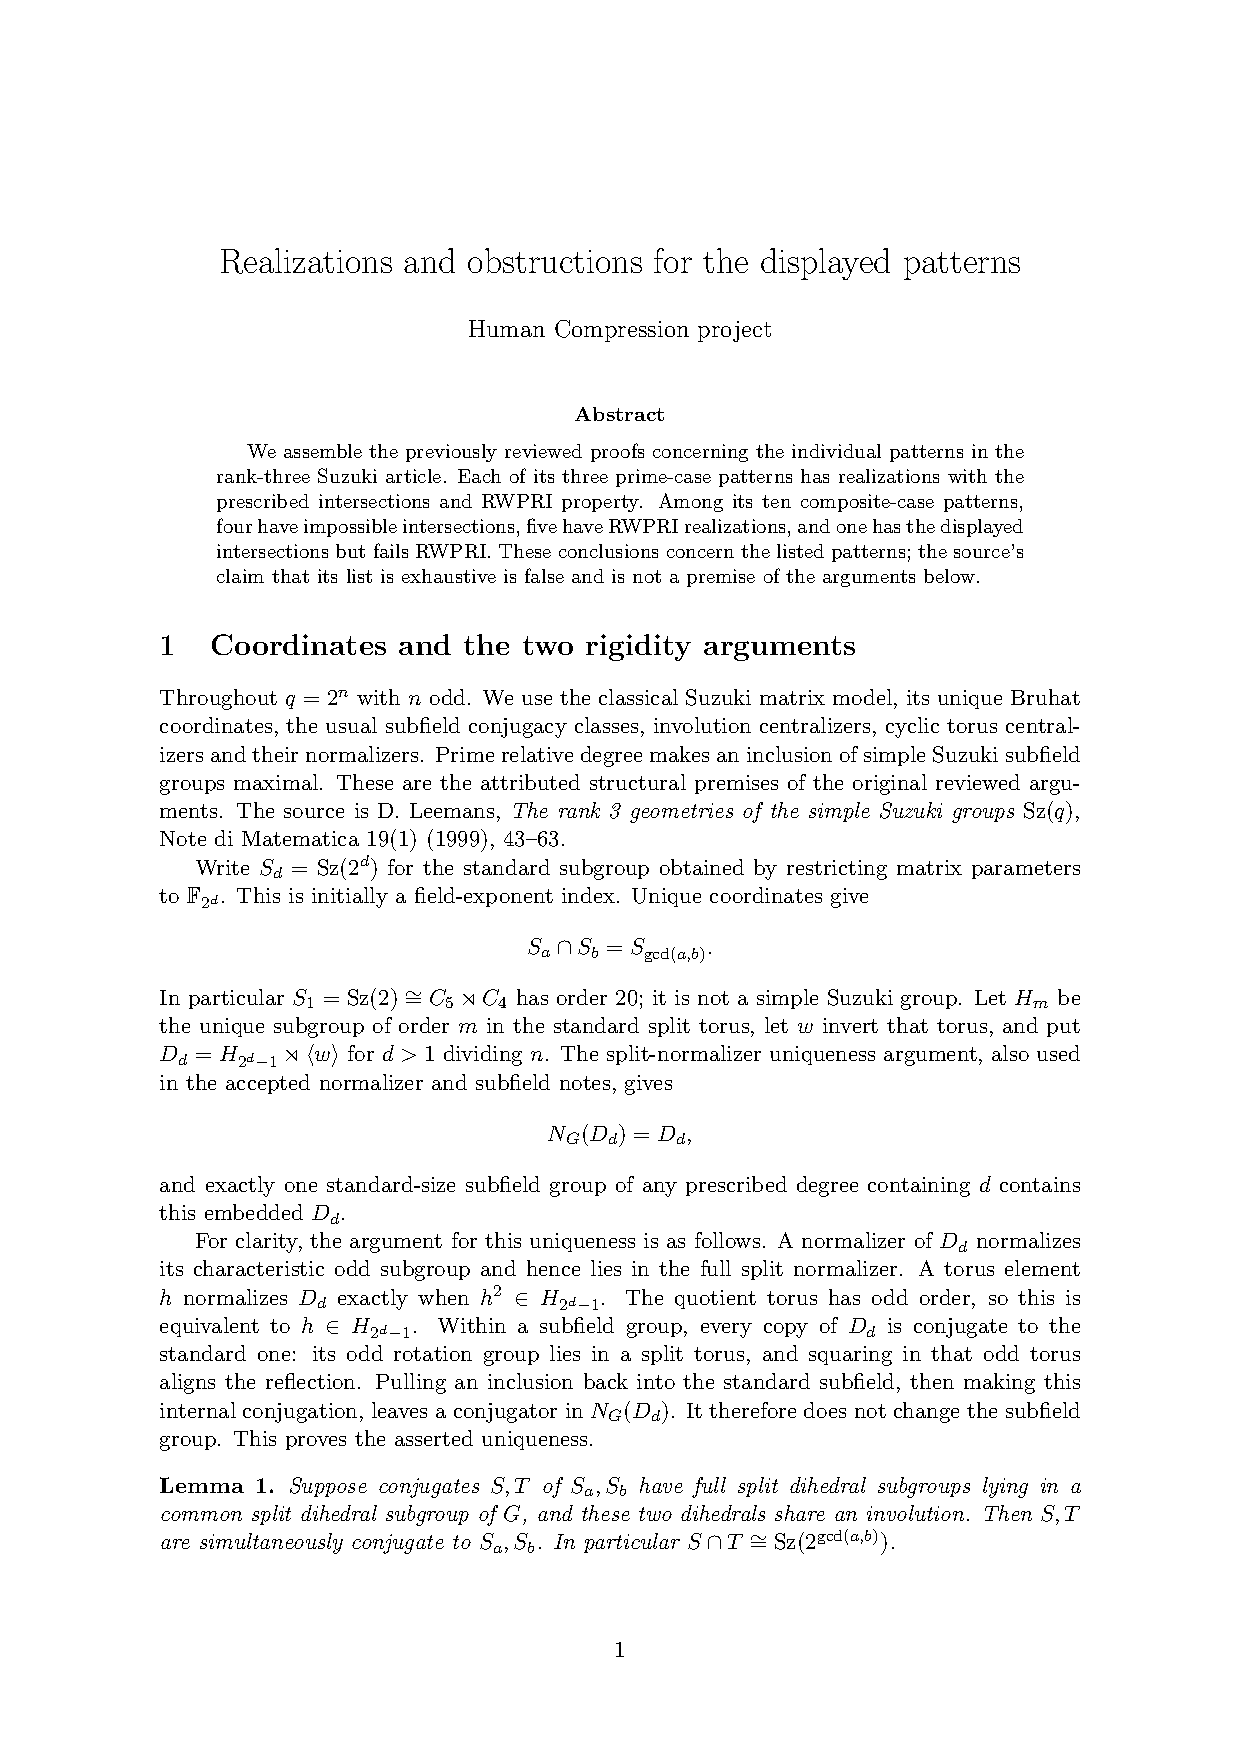
\includepdf[pages=-]{proofs/realizations.pdf}
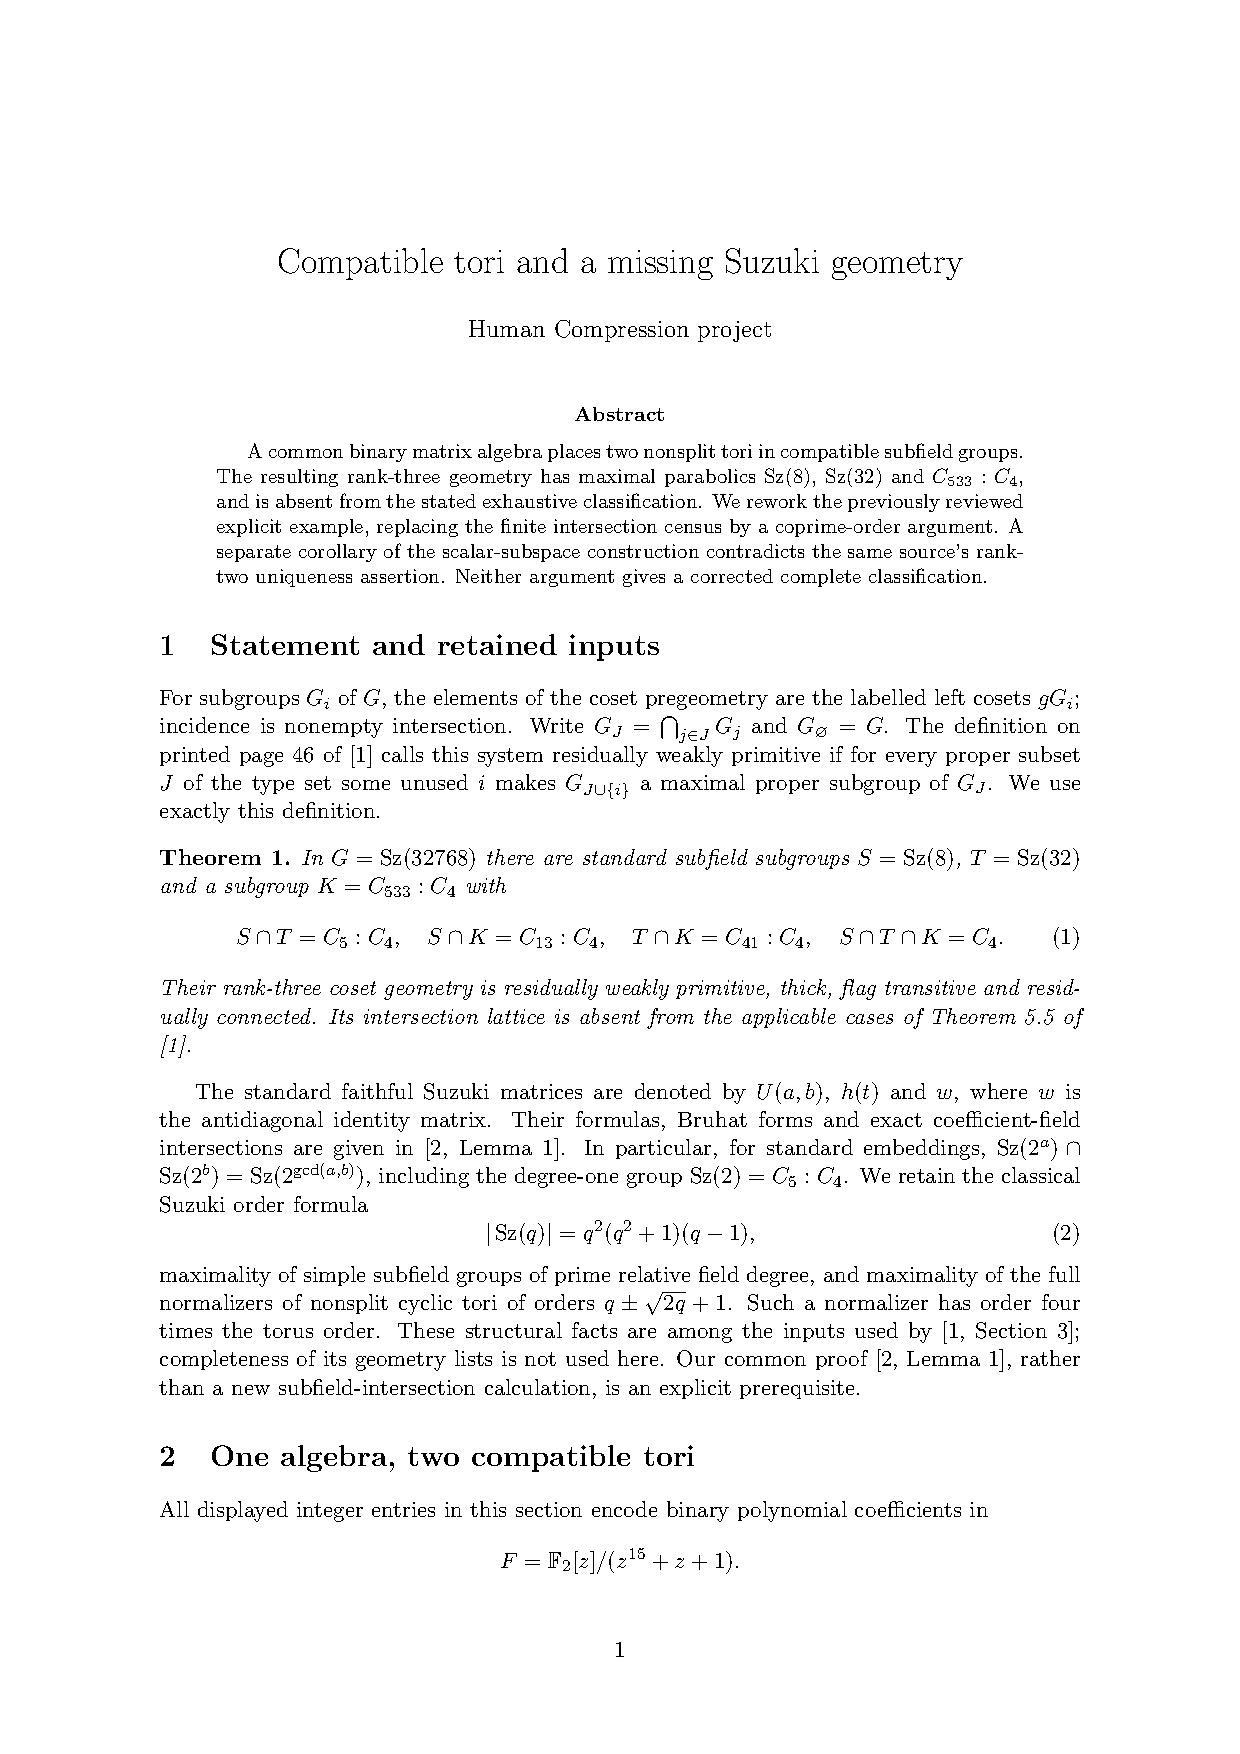
\includepdf[pages=-]{proofs/principal.pdf}
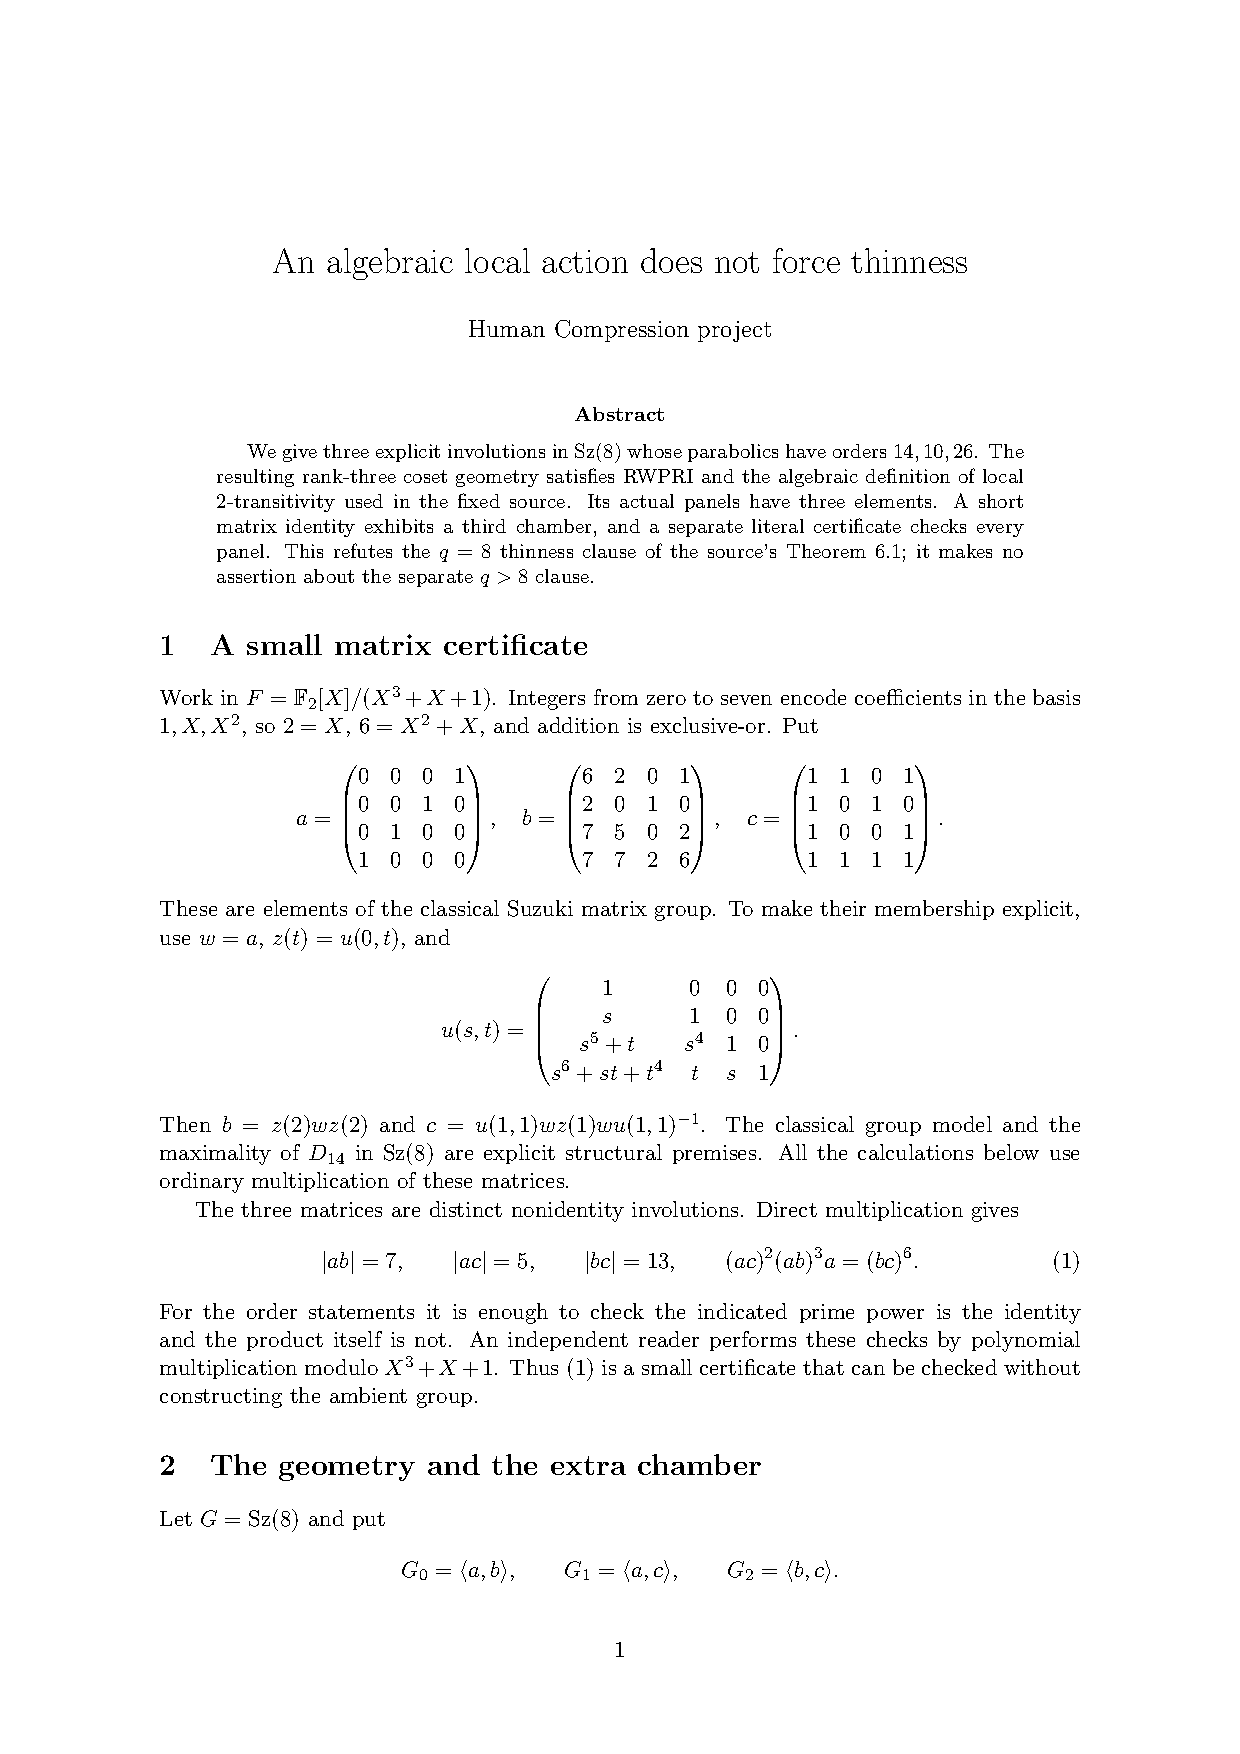
\includepdf[pages=-]{proofs/nonthin8.pdf}
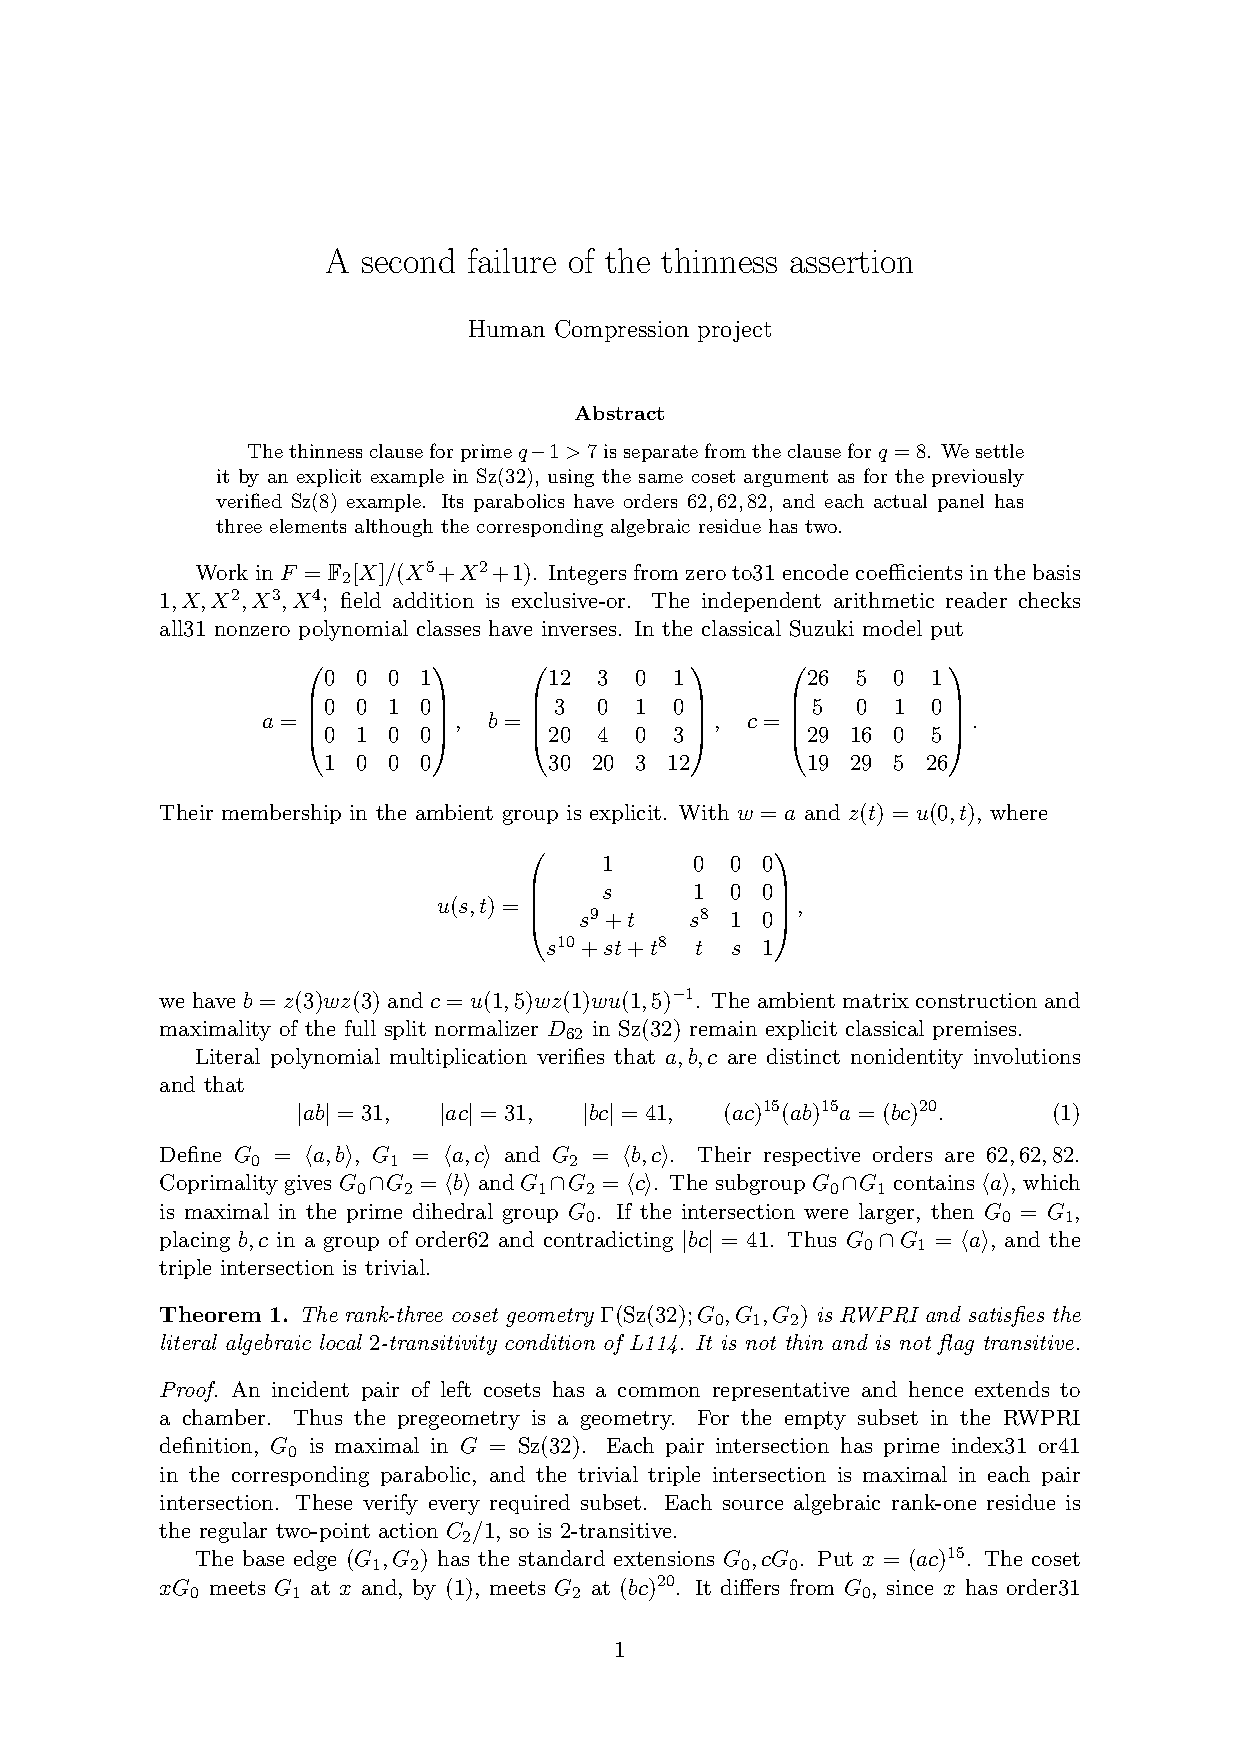
\includepdf[pages=-]{proofs/nonthin32.pdf}
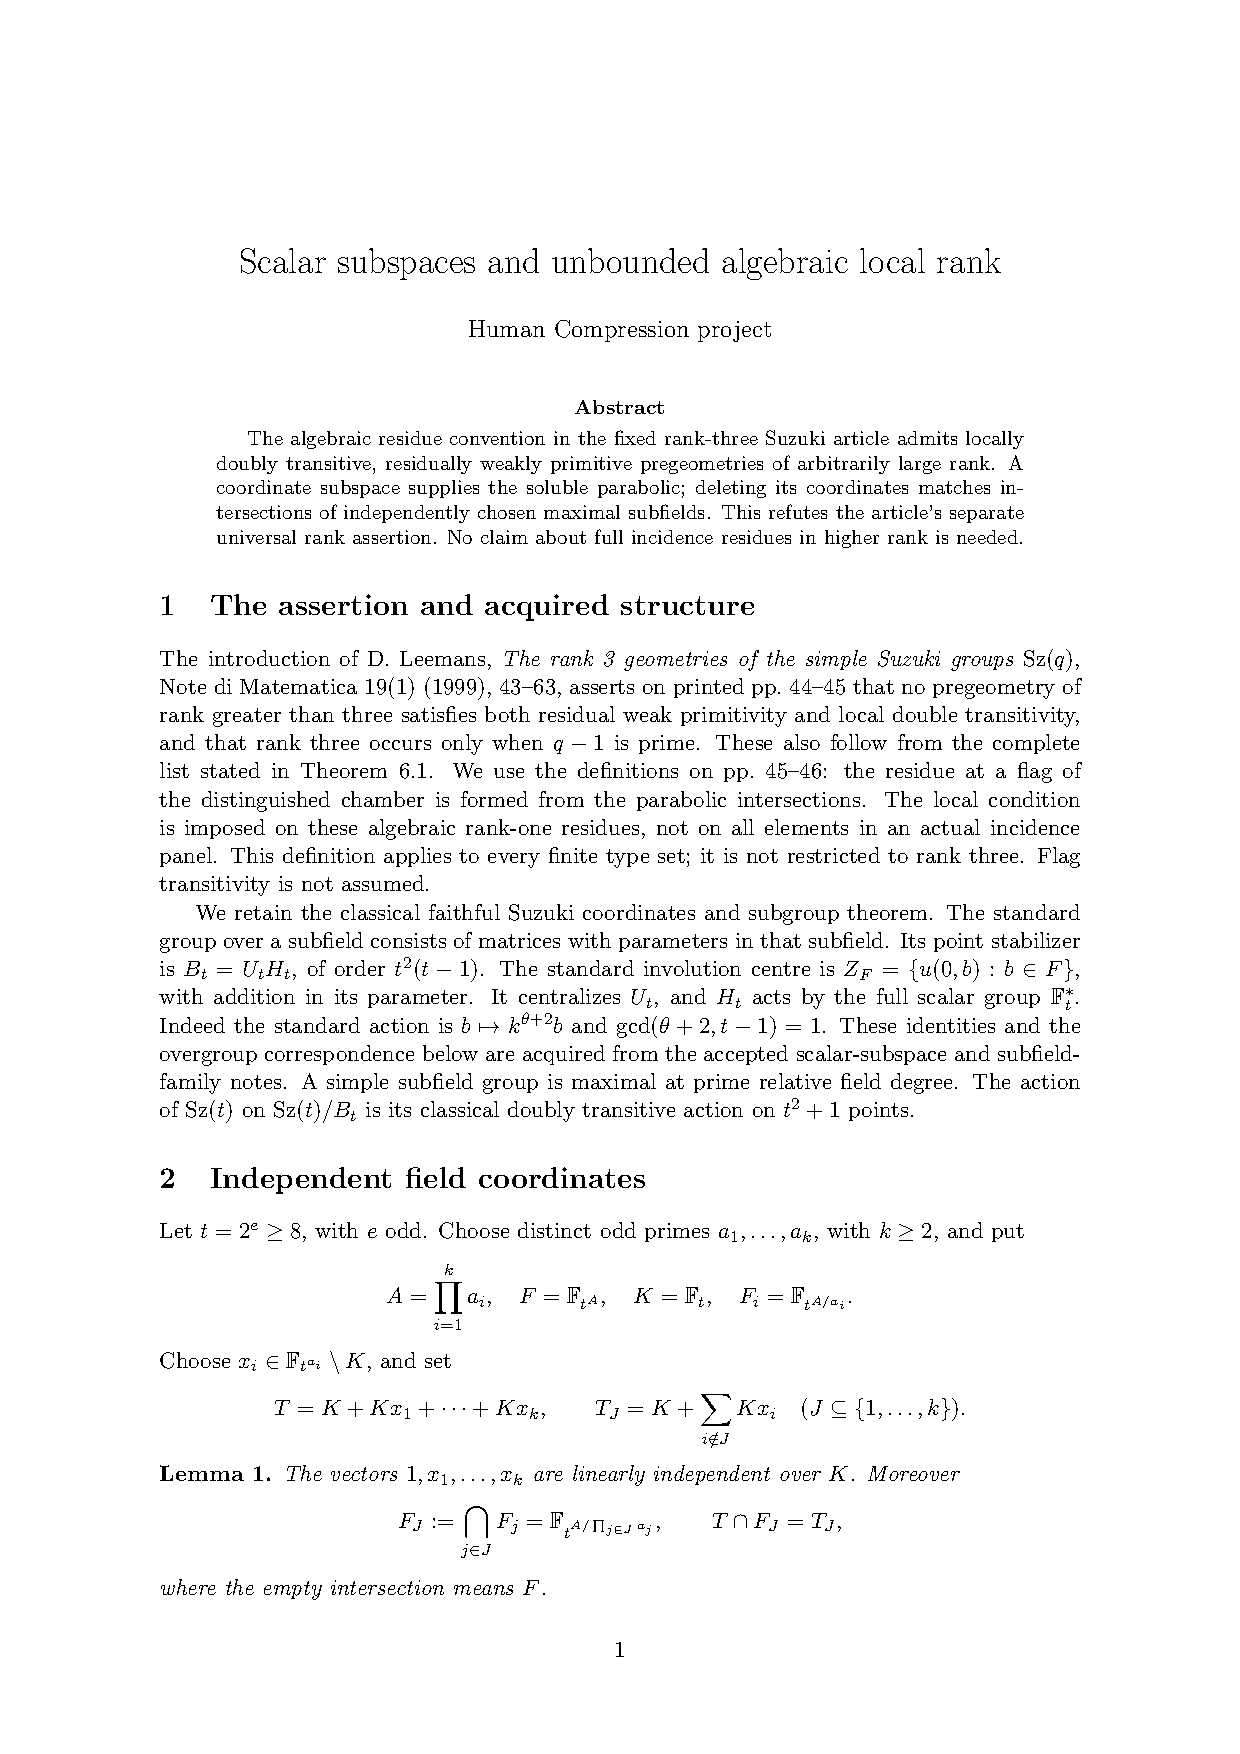
\includepdf[pages=-]{proofs/local_rank.pdf}
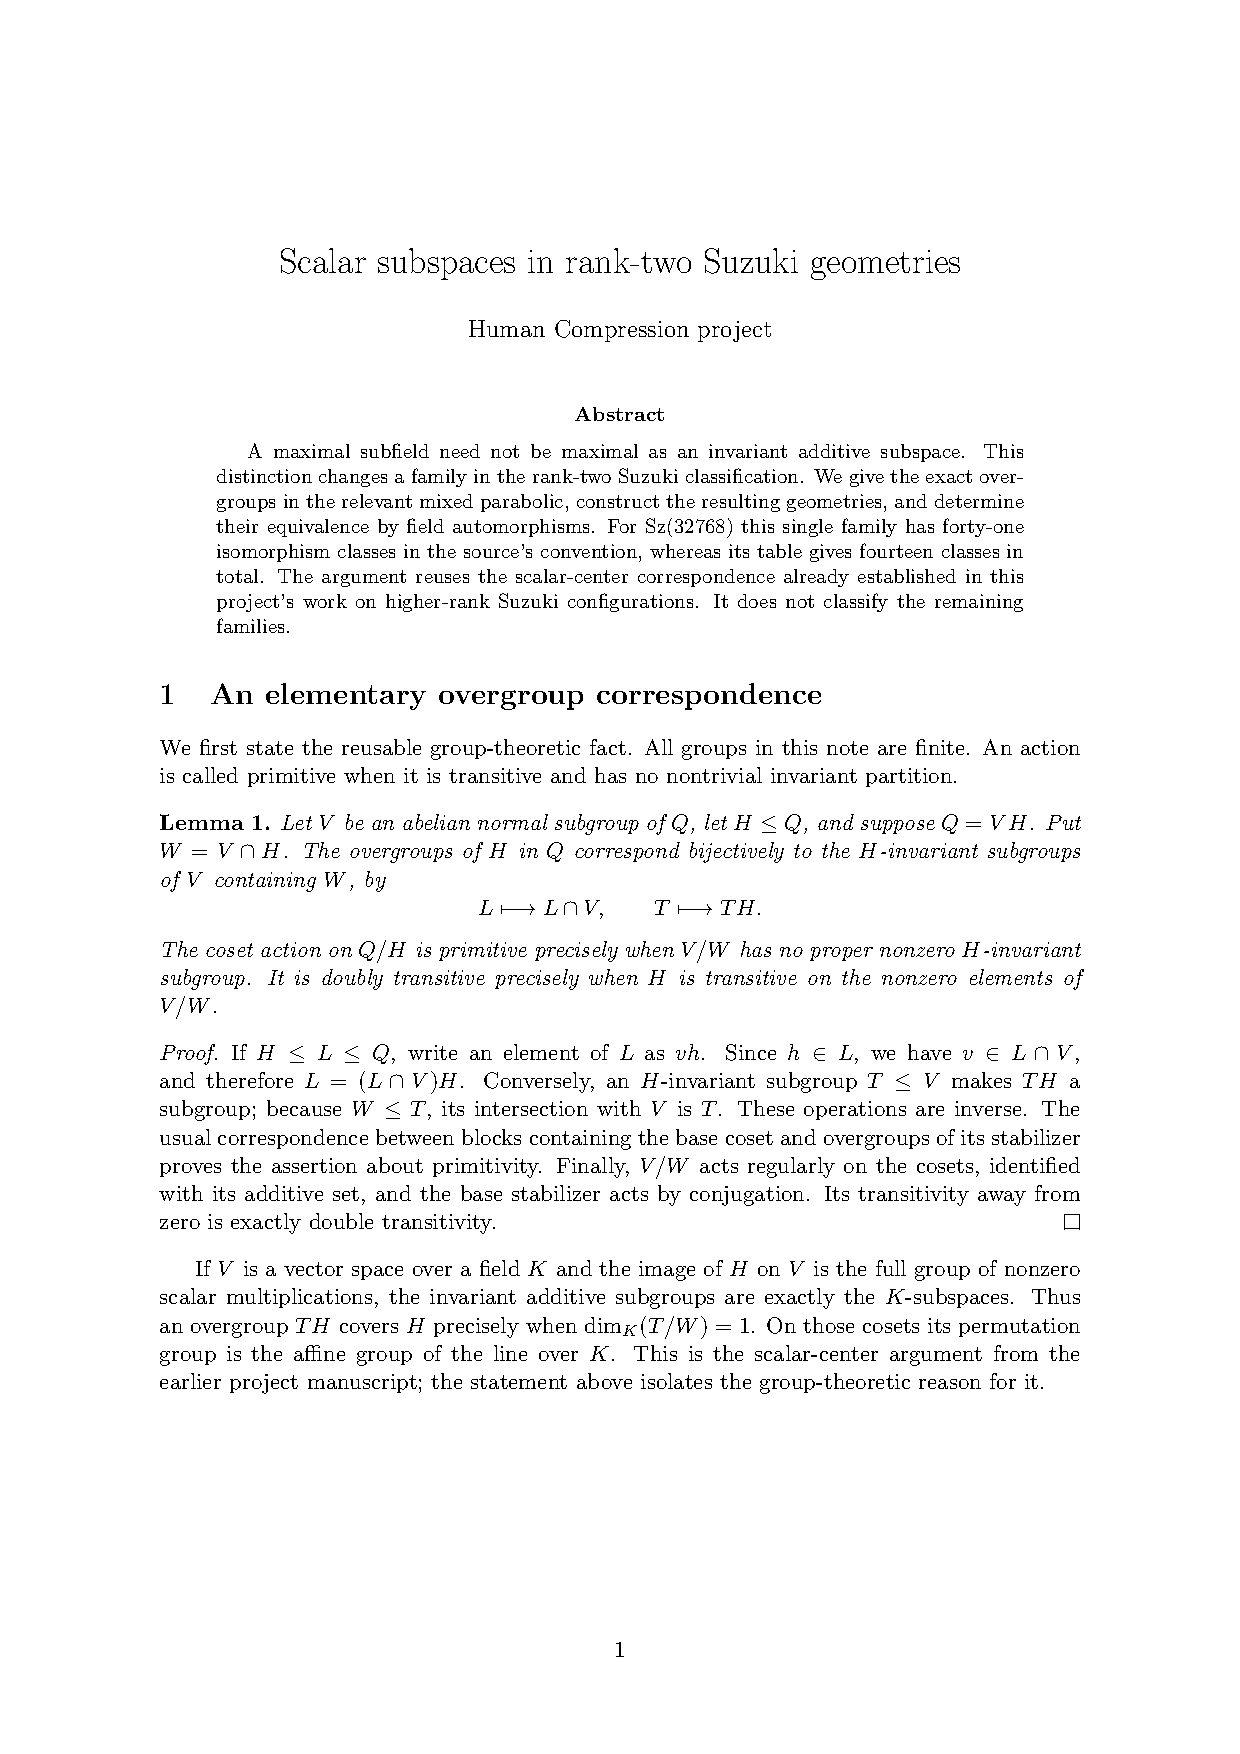
\includepdf[pages=-]{proofs/scalar_subspaces.pdf}
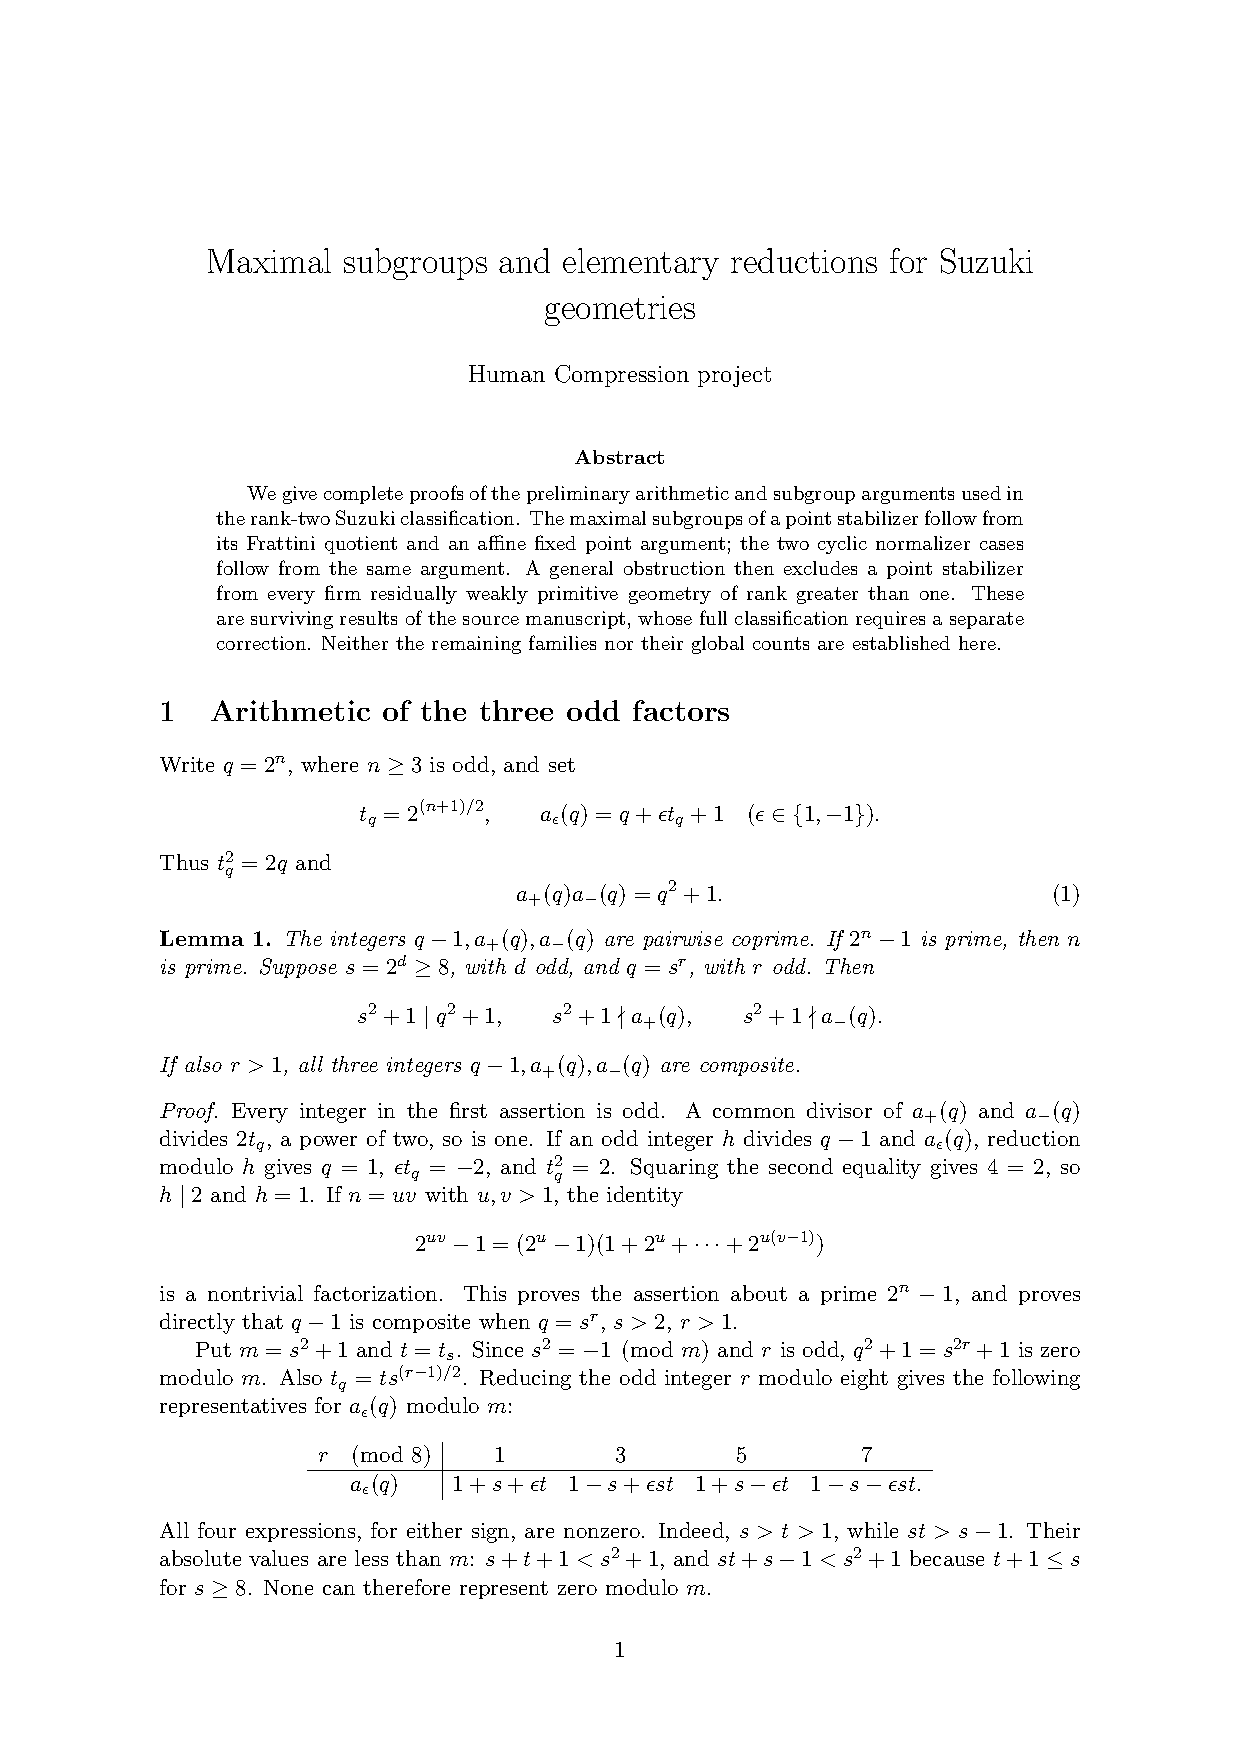
\includepdf[pages=-]{proofs/common_preliminaries.pdf}
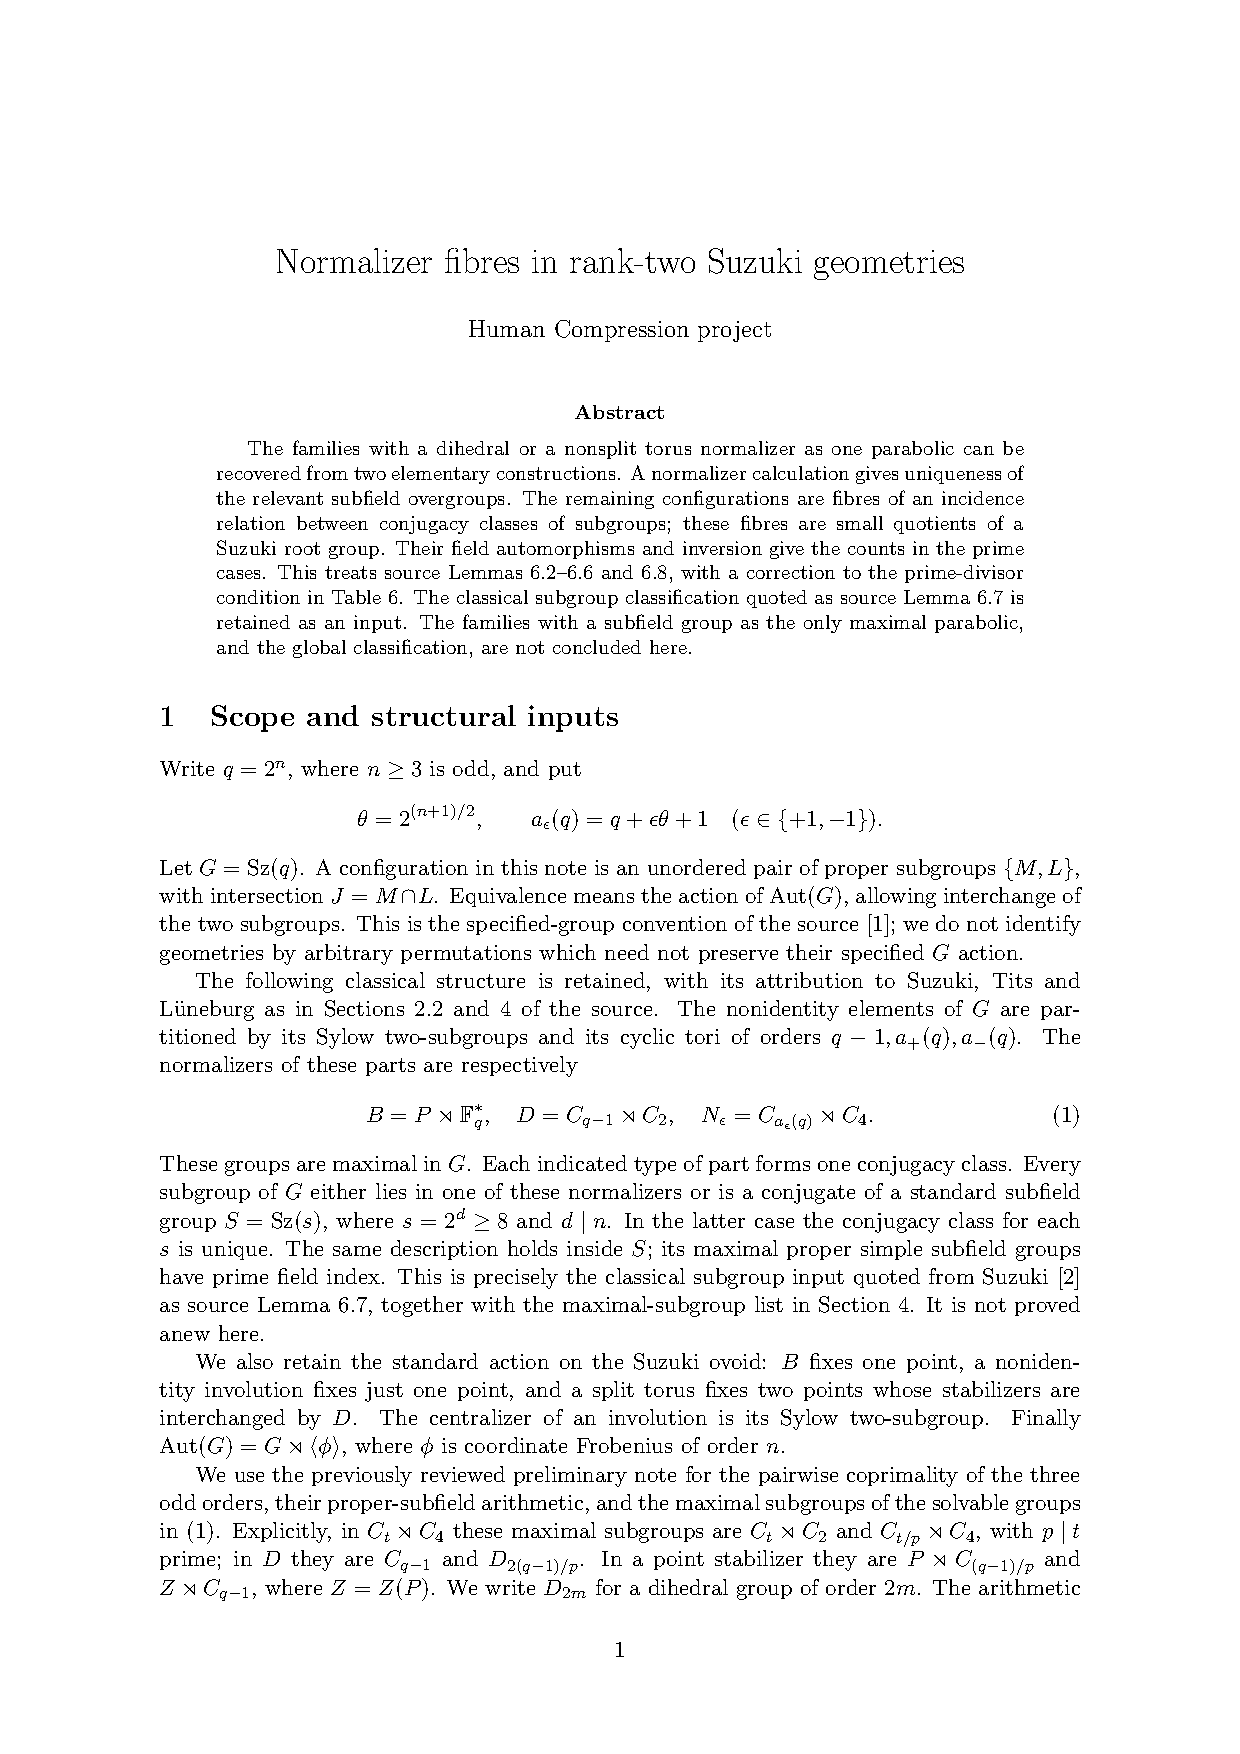
\includepdf[pages=-]{proofs/normalizer_families.pdf}
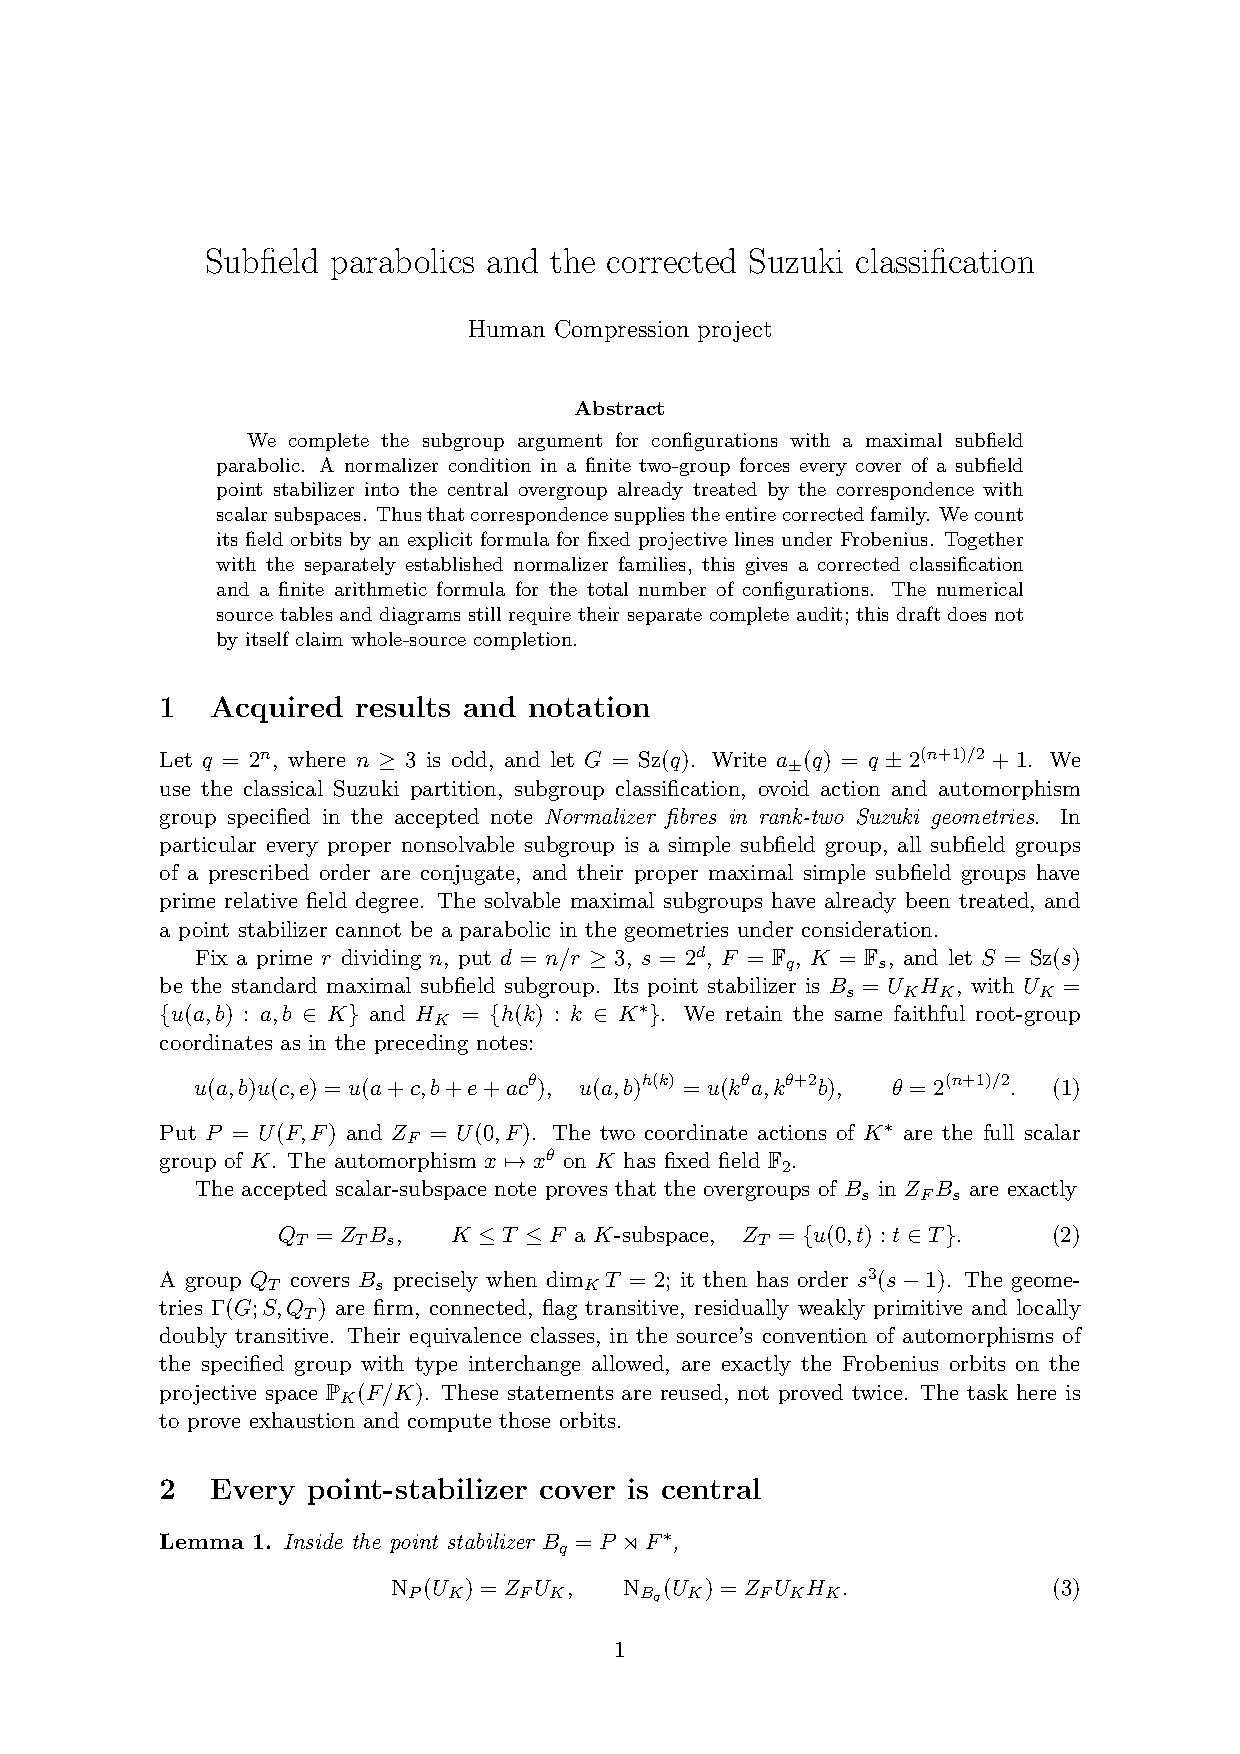
\includepdf[pages=-]{proofs/subfield_families.pdf}
\end{document}
